
%% Customizações do abnTeX2 (http://www.abntex.net.br) para o Instituto de Matemática,
%% Estatística e Computação Científica da Universidade Estadual de Campinas (IMECC-UNICAMP)
%%
%% This work may be distributed and/or modified under the conditions of the LaTeX Project
%% Public License, either version 1.3 of this license or (at your option) any later version.
%% The latest version of this license is in http://www.latex-project.org/lppl.txt and version
%% 1.3 or later is part of all distributions of LaTeX version 2005/12/01 or later.
%%
%% This work has the LPPL maintenance status `maintained'.
%% 
%% The Current Maintainer of this work is Fábio Rodrigues Silva, gfabinhomat@gmail.com
%%
%% Further information about abnTeX2 are available on http://www.abntex.net.br
%%
\documentclass[
	oldfontcommands,
	% -- opções de customização --
	sumario=tradicional,
	%sumario=abnt-6027-2012,
	% -- opções da classe memoir --
	12pt,			% tamanho da fonte
	openright,		% capítulos começam em pág ímpar (insere página vazia caso preciso)
	oneside,		% para impressão em verso e anverso. Oposto a 'oneside'
	a4paper,		% tamanho do papel. 
	% -- opções da classe abntex2 --
	%chapter=TITLE,		% títulos de capítulos convertidos em letras maiúsculas
	%section=TITLE,		% títulos de seções convertidos em letras maiúsculas
	%subsection=TITLE,	% títulos de subseções convertidos em letras maiúsculas
	%subsubsection=TITLE,	% títulos de subsubseções convertidos em letras maiúsculas
	% -- opções do pacote babel --
	english,		% idioma adicional para hifenização
	brazil			% o último idioma é o principal do documento
	]{imecc-unicamp}
% ----------------------------------------------------------
% PACOTES ESSENCIAIS
% Aqui você pode adicionar seus pacotes específicos para uso em seu trabalho.
% Em PACOTES PESSOAIS insira os pacotes que desejar.
% ----------------------------------------------------------
% PACOTES BÁSICOS (ESSENCIAIS AO MODELO)
\usepackage{lmodern}			% Usa a fonte Latin Modern
\usepackage[T1]{fontenc}		% Selecao de codigos de fonte.
\usepackage[utf8]{inputenc}		% Codificacao do documento (conversão automática dos acentos)
\usepackage{lastpage}			% Usado pela Ficha catalográfica
\usepackage{indentfirst}		% Indenta o primeiro parágrafo de cada seção.
\usepackage{color,xcolor}		% Controle das cores
\usepackage{graphicx}			% Inclusão de gráficos
\usepackage{microtype} 			% para melhorias de justificação
\usepackage{amssymb}
\usepackage{listings}
% ----------------------------------------------------------
% ----------------------------------------------------------
% PACOTES PARA GLOSSÁRIO
\usepackage[subentrycounter,seeautonumberlist,nonumberlist=true]{glossaries}
% para usar o xindy ao invés do makeindex:
%\usepackage[xindy={language=portuguese},subentrycounter,seeautonumberlist,nonumberlist=true]{glossaries}
% ----------------------------------------------------------
% ----------------------------------------------------------
% PACOTES DE CITAÇÕES (PRINCIPAIS PACOTES DO MODELO)
\usepackage[brazilian]{backref}		% Paginas com as citações na bibl
\usepackage[alf,
	    abnt-repeated-author-omit=yes,
	    abnt-etal-list=0]{abntex2cite}		% Citações padrão ABNT
% É possível utilizar o sistema numérico de chamada, alterando a opção 'alf' para 'num'.
% Outros estilos bibliográficos podem ser usados. Se este for o caso, comente o pacote acima
% e utilize, por exemplo, o comando abaixo
% \bibliographystyle{acm}
% Consulte outros estilos de bibliografia consultando o manual de estilos bibliográficos do
% BibTeX em 'http://www.bibtex.org/'
% ----------------------------------------------------------
% ----------------------------------------------------------
% PACOTES ADICIONAIS (usados apenas no âmbito do Modelo Canônico do abnteX2)
\usepackage{lipsum}			% para geração de dummy text
% ----------------------------------------------------------
% ----------------------------------------------------------
% PACOTES PESSOAIS (USADOS PELO AUTOR -- acrescente aqui seus pacotes)
% ----------------------------------------------------------
\usepackage[portuguese,onelanguage]{algorithm2e}	% para inserir algoritmos (longend,vlined)
% \usepackage{amsbsy}			% para símbolos matemáticos em negrito
% \usepackage{amscd}			% para diagramas
% \usepackage{amsfonts}			% fontes AMS
% \usepackage{amsmath}			% facilidades matemáticas
% \usepackage{amssymb}			% para os símbolos mais antigos
% \usepackage{amstext}			% para fragmentos tipo texto em modo matemático
\usepackage{amsthm}			% para teoremas
\usepackage{hyperref}			% Amplo suporte para hipertexto em LaTeX
\usepackage{cleveref}			% Referência cruzada inteligente
\usepackage{dsfont}			% para o estilo de conjuntos de números $\mathds{R}$
% \usepackage{ifthen}			% comandos de condição em LaTeX
\usepackage{listings}           	% para inserir códigos de outras linguagens de programação
% \usepackage{lscape}             	% para imprimir alguma página no formato paisagem
\usepackage{mathabx}			% conjunto de simbolos matemáticos
% \usepackage{mathrsfs}			% suporte para fontes RSFS
% \usepackage{pdfpages}           	% para inserir páginas PDF no texto

% \usepackage{verbatim}
\usepackage[a4paper,
            left=3cm,
            right=2cm,
            top=3cm,
            bottom=2cm]{geometry}


\usepackage[scaled]{helvet}
\renewcommand{\familydefault}{\sfdefault}

\usepackage{titlesec}
\usepackage{placeins}
% ----------------------------------------------------------
\renewcommand{\ABNTEXchapterfont}{\normalfont\bfseries}
\renewcommand{\ABNTEXsectionfont}{\normalfont\bfseries}
\renewcommand{\ABNTEXsubsectionfont}{\normalfont\bfseries}

% ----------------------------------------------------------
% ----------------------------------------------------------
% INFORMAÇÕES E DADOS PARA CAPA E FOLHA DE ROSTO
% ----------------------------------------------------------
% Os comandos abaixo devem ser preenchidos em língua PORTUGUESA
\titulo{Título do seu Trabalho Acadêmico:\\ dissertação de mestrado ou tese de doutorado}
\tipotrabalho{Dissertação}
% \tipotrabalho{Tese}
% \curso{Estatística}
% \curso{Matemática}
% \curso{Matemática Aplicada}
\curso{Matemática Aplicada e Computacional}
% \curso{}  % Se for aluno do PROFMAT
% ----------------------------------------------------------
% ----------------------------------------------------------
% Os comandos abaixo devem ser preenchidos na língua DO TRABALHO
% ---
% Se autor do sexo MASCULINO
% \autor{Nome Completo do Aluno}
% \titulacao{Mestre}
% \titulacao{Doutor}
% ---
% Se autor do sexo FEMININO, descomente e preencha os campos abaixo
\autor[autora]{Nome Completo da Aluna}
\titulacao{Mestra}
% \titulacao{Doutora}
% ---
% Se orientador/coorientador do sexo MASCULINO
% \orientador{Nome Completo do Orientador}
% \coorientador{Nome Completo do Coorientador}
% ---
% Se orientador/coorientador do sexo FEMININO, descomente e preencha os campos abaixo (exceto se o trabalho for em inglês)
\orientador[Orientadora]{Nome Completo da Orientadora}
\coorientador[Coorientadora]{Nome Completo da Coorientadora}
% ---
\data{Ano}
% ---
% Se seu trabalho for em língua NÃO portuguesa, descomente e preencha os campos abaixo na lingua DO TRABALHO
% \setboolean{ABNTEXotherlanguage}{true}
% \titulootherlang{Title of your Academic Work:\\ master thesis or phd thesis}
% \cursootherlang{Statistics}
% \cursootherlang{Mathematics}
% \cursootherlang{Applied Mathematics}
% \cursootherlang{Computational and Applied Mathematics}
% \typework{Dissertation}
% \typework{Thesis}
% \titulation{Master}
% \titulation{Doctor}
% ---
% No caso de Cotutela Internacional de Tese, descomente e preencha os campos abaixo
% \setboolean{ABNTEXcotutela}{true}
% \universidadecotutela{NAME OF THE UNIVERSITY}
% \paiscotutela{COUNTRY}
% ----------------------------------------------------------
% ----------------------------------------------------------
% ----------------------------------------------------------
% CONFIGURAÇÕES GERAIS
% As configurações gerais são colocadas aqui, como novos comandos para o corpo do texto,
% informações de bookmark para o PDF, tamanho de parágrafos, entre outros.

% ----------------------------------------------------------
% Configurações do pacote BACKREF
% ----------------------------------------------------------
% Usado sem a opção hyperpageref de backref
\renewcommand{\backrefpagesname}{Citado na(s) página(s):~}
% Texto padrão antes do número das páginas
\renewcommand{\backref}{}
% Define os textos da citação
\renewcommand*{\backrefalt}[4]{
	\ifcase #1 %
		Nenhuma citação no texto.%
	\or
		Citado na página #2.%
	\else
		Citado #1 vezes nas páginas #2.%
	\fi}%
% ---

% ----------------------------------------------------------
% \theoremstyle{plain}
\newtheorem{theorem}{Teorema}%[chapter]
\newtheorem{lemma}{Lema}%[chapter]
\providecommand*{\lemmaautorefname}{Lema}
\newtheorem{proposition}{Proposição}%[chapter]
\providecommand*{\propositionautorefname}{Proposição}
\newtheorem{corollary}{Corolário}%[chapter]
\providecommand*{\corollaryautorefname}{Corolário}
\newtheorem{conjecture}{Conjectura}%[chapter]
\providecommand*{\conjectureautorefname}{Conjectura}
\newtheorem{definition}{Definição}%[chapter]
\providecommand*{\definitionautorefname}{Definição}
\newtheorem{notation}{Notação}%[chapter]
\providecommand*{\notationautorefname}{Notação}
\newtheorem{remark}{Observação}%[chapter]
\providecommand*{\remarkautorefname}{Observação}
\newtheorem{example}{Exemplo}%[chapter]
\providecommand*{\exampleautorefname}{Exemplo}
\newtheorem{note}{Nota}%[chapter]
\providecommand*{\noteautorefname}{Nota}
% ----------------------------------------------------------

% ----------------------------------------------------------
% Conjunto de configuracoes para o pacote 'listings'
% ----------------------------------------------------------
\lstset{
  language=C++,
  basicstyle=\ttfamily, 
  keywordstyle=\color{blue}, 
  stringstyle=\color{verde}, 
  commentstyle=\color{red}, 
  extendedchars=true, 
  showspaces=false, 
  showstringspaces=false,
  numbers=left,
  numberstyle=\tiny,
  breaklines=true, 
  backgroundcolor=\color{green!10},
  breakautoindent=true,
  fontadjust=false
}
% ----------------------------------------------------------

% ----------------------------------------------------------
% Informações do PDF
% ----------------------------------------------------------
% Configurações de aparência do PDF final
% ---
% alterando o aspecto da cor azul
\definecolor{blue}{RGB}{41,5,195}
\definecolor{verde}{rgb}{0,0.5,0}
% ---
\makeatletter
\hypersetup{
  %pagebackref=true,
  pdftitle={\@title},
  pdfauthor={\@author},
  pdfsubject={%
    \imprimirtipotrabalho\ apresentada ao Instituto de Matemática, Estatística %
    e Computação Científica da Universidade Estadual de Campinas como parte dos %
    requisitos exigidos para a obtenção do título de \imprimirtitulacao\ em %
    \imprimircurso.
  },
  pdfcreator={LaTeX with unicamp-abnTeX2},
  pdfkeywords={abnt}{latex}{abntex}{abntex2}{trabalho acadêmico},
  colorlinks=true,		% false: boxed links; true: colored links
  linkcolor=blue,		% color of internal links
  citecolor=blue,		% color of links to bibliography
  filecolor=magenta,		% color of file links
  urlcolor=blue,		% color of internet links
  bookmarksdepth=4
}
\makeatother
% ----------------------------------------------------------

% ----------------------------------------------------------
% COMANDOS GLOBAIS
% ----------------------------------------------------------
\everymath{\displaystyle}
% ---
\renewcommand{\sin}{\mathrm{sen}}
\renewcommand{\tan}{\mathrm{tg}}
\renewcommand{\csc}{\mathrm{cossec}}
\renewcommand{\cot}{\mathrm{cotg}}
% ---
\DeclareMathOperator{\posto}{\mathrm{posto}}
\DeclareMathOperator{\conv}{\mathrm{conv}}
\DeclareMathOperator{\diag}{\mathrm{diag}}
\DeclareMathOperator{\argmin}{\mathrm{arg}\min}
\DeclareMathOperator{\argmax}{\mathrm{arg}\max}
% ---
% O tamanho do parágrafo é dado por:
\setlength{\parindent}{2.0cm}
% Controle do espaçamento entre um parágrafo e outro:
\setlength{\parskip}{0.2cm}  % tente também \onelineskip
% ---
% Para que apareça o nome 'Capítulo X' antes do título de cada capítulo
% \chapterstyle{default}
% ----------------------------------------------------------
\newsubfloat{figure}% Allow subfloats in figure environment
\providecommand*{\subfigureautorefname}{Subfigura}

\lstdefinestyle{custompython}{
    language=Python,
    backgroundcolor=\color{gray!5},
    keywordstyle=\color{blue}\bfseries,
    commentstyle=\color{gray!50},
    stringstyle=\color{red},
    basicstyle=\ttfamily\small,
    frame=single,
    showstringspaces=false,
    tabsize=4,
    captionpos=b,
    numbers=left,
    numberstyle=\tiny\color{gray},
}

% \chapter - tamanho 12pt, negrito
\titleformat{\chapter}[hang]
  {\bfseries\fontsize{12pt}{14pt}\selectfont}
  {\thechapter.}{1em}{\MakeUppercase}
\titlespacing*{\chapter}{0pt}{0pt}{12pt}

% \section - tamanho 12pt, negrito
\titleformat{\section}
  {\bfseries\fontsize{12pt}{14pt}\selectfont}
  {\thesection}{1em}{}
\titlespacing*{\section}{0pt}{6pt}{6pt}

% \subsection - tamanho 12pt, negrito
\titleformat{\subsection}
  {\bfseries\fontsize{12pt}{14pt}\selectfont}
  {\thesubsection}{1em}{}


\renewcommand{\ABNTEXchapterfont}{\bfseries\MakeUppercase\Large}
\renewcommand{\ABNTEXsectionfont}{\bfseries\large}
\renewcommand{\ABNTEXsubsectionfont}{\bfseries\normalsize}


\renewcommand{\ABNTEXchapterfontsize}{\normalsize}
\renewcommand{\ABNTEXsectionfontsize}{\normalsize}
\renewcommand{\ABNTEXsubsectionfontsize}{\normalsize}

% Se quiser tirar a caixa alta dos títulos do sumário (opcional)
\renewcommand{\ABNTEXchapterfont}{\normalfont}
\renewcommand{\ABNTEXsectionfont}{\normalfont}
\renewcommand{\ABNTEXsubsectionfont}{\normalfont}
% ----------------------------------------------------------
% ----------------------------------------------------------
% COMPILA O ÍNDICE (OPCIONAL)
\makeindex
% ----------------------------------------------------------
% ----------------------------------------------------------
% -----------------------------------------------------------------------------------------------
% %%%%%%%%%%%%%%%%%%%%%%%%%%%%%%%%%%%%% INÍCIO DO DOCUMENTO %%%%%%%%%%%%%%%%%%%%%%%%%%%%%%%%%%%%%
% -----------------------------------------------------------------------------------------------
\begin{document}
% Seleciona o idioma do documento (conforme pacotes do babel)
\selectlanguage{brazil}
% \selectlanguage{english}
% Retira espaço extra obsoleto entre as frases.
\frenchspacing
% ---------------------------------------------------------------------------------
% %%%%%%%%%%%%%%%%%%%%%%% INÍCIO DOS ELEMENTOS PRÉ-TEXTUAIS %%%%%%%%%%%%%%%%%%%%%%%
% ---------------------------------------------------------------------------------
\pretextual
% ----------------------------------------------------------
% PRIMEIRA FOLHA (OBRIGATÓRIO)
\imprimirprimeirafolha
% ----------------------------------------------------------
% ----------------------------------------------------------
% FOLHA DE ROSTO (OBRIGATÓRIO)
% ---
% Após realizar as correções finais de seu trabalho acadêmico, escaneie a folha de rosto
% devidamente assinada pelo orientador e salve no formato PDF com o nome 'folha-de-rosto.pdf'
% no diretório do seu projeto. Daí substitua a linha do comando '\imprimirfolhaderosto'
% pelas 3 linhas de comando abaixo:
% ---
% \begin{folhaderosto}
%     \includepdf{folha-de-rosto.pdf}
% \end{folhaderosto}
% ---
\imprimirfolhaderosto

% ----------------------------------------------------------
% ----------------------------------------------------------
% FICHA CATALOGRÁFICA (OBRIGATÓRIO)
% ---
% A biblioteca da UNICAMP lhe fornecerá um PDF com a ficha catalográfica definitiva após a defesa
% do trabalho {http://hamal.bc.unicamp.br/catalogonline2/}. Quando estiver com o documento, salve-o
% como PDF no diretório do seu projeto e deixe apenas o comando '\includepdf{ficha-catalografica.pdf}'
% dentro do ambiente abaixo
% ---
% \begin{fichacatalografica}
%     \begin{center}
% 	{\ABNTEXchapterfont\large A ficha catalográfica será fornecida pela biblioteca}
%     \end{center}
% %     \includepdf{ficha-catalografica.pdf}
% \end{fichacatalografica}
% ----------------------------------------------------------
% ----------------------------------------------------------
% FOLHA DE APROVAÇÃO (OBRIGATÓRIO)
% ---
% A folha de aprovação será fornecida pela secretaria de pós-graduação. Após recebê-la, escaneie a folha
% salvando em PDF no diretório do seu projeto com o nome 'folhadeaprovacao.pdf' e deixe apenas o comando
% '\includepdf{folhadeaprovacao.pdf}' dentro do ambiente abaixo
% ---
% \begin{folhadeaprovacao}
%     \centering{\ABNTEXchapterfont\large A folha de aprovação será fornecida pela Secretaria de Pós-Graduação}
% %     \includepdf{folhadeaprovacao.pdf}
% \end{folhadeaprovacao}
% ----------------------------------------------------------
% ----------------------------------------------------------
% DEDICATÓRIA (OPCIONAL)
% \begin{dedicatoria}
%    \vspace*{\fill}
%    \centering
%    \noindent
%    \textit{
%       Este trabalho é dedicado às crianças adultas que,\\
%       quando pequenas, sonharam em se tornar cientistas.
%    }
%    \vspace*{\fill}
% \end{dedicatoria}
% ----------------------------------------------------------
% ----------------------------------------------------------
% AGRADECIMENTOS (OPCIONAL)
% \begin{agradecimentos}
% Inserir os agradecimentos, sem esquecer dos órgãos de fomento!
% \end{agradecimentos}
% ----------------------------------------------------------
% ----------------------------------------------------------
% EPÍGRAFE (OPCIONAL)
% \begin{epigrafe}
%     \vspace*{\fill}
%     \begin{flushright}
% 	\textit{``Não vos amoldeis às estruturas deste mundo, \\
% 	    mas transformai-vos pela renovação da mente, \\
% 	    a fim de distinguir qual é a vontade de Deus: \\
% 	    o que é bom, o que Lhe é agradável, o que é perfeito.\\
% 	    (Bíblia Sagrada, Romanos 12, 2)
% 	}
%     \end{flushright}
% \end{epigrafe}
%
%
% ----------------------------------------------------------
% ----------------------------------------------------------
% RESUMOS (OBRIGATÓRIO)
%% -------------------------------------------------------------
%  RESUMOS
\setlength{\absparsep}{18pt} % ajusta o espaçamento dos parágrafos do resumo
% -------------------------------------------------------------
% ATENÇÃO: o ambiente 'otherlanguage*' deve ser usado para o resumo que não está na
% língua vernácula do trabalho, com a respectiva opção linguística do pacote 'babel'.
% -------------------------------------------------------------
% resumo em PORTUGUÊS (OBRIGATÓRIO)
\begin{center}
    \textbf{RESUMO}
\end{center}

\begin{otherlanguage*}{brazil}
    Este trabalho investiga diferentes formas de estruturação do problema de 
    Geração Procedural de Conteúdo (PCG) utilizando algoritmos de Aprendizado por 
    Reforço (RL), com foco na criação de fases em formato de labirinto. Foram 
    exploradas múltiplas representações do espaço de estados e ações, diferentes 
    configurações de recompensas e cenários com variações de parâmetros ambientais. 
    O objetivo foi compreender como essas decisões de modelagem influenciam o 
    comportamento e desempenho dos agentes geradores. Para isso, foram implementados 
    experimentos com o algoritmo Proximal Policy Optimization (PPO), analisando sua 
    capacidade de aprender padrões válidos e diversificados de geração, mesmo sem 
    convergir para uma política ótima. Os resultados demonstram que a escolha da 
    representação e da recompensa impacta diretamente na qualidade e diversidade dos 
    conteúdos gerados, sendo também um desafio traduzir percepções humanas visuais em 
    métricas computacionais claras. A pesquisa contribui para a compreensão das 
    limitações e possibilidades do uso de RL no contexto de PCG, oferecendo direções 
    para futuros estudos que visem otimizar o processo de geração de conteúdo em jogos 
    digitais.

    \textbf{Palavras-chave}: RL. PCG. Geração procedural de conteúdo em jogos.
\end{otherlanguage*}
% -------------------------------------------------------------
% -------------------------------------------------------------
% resumo em INGLÊS (OBRIGATÓRIO)
\newpage
\begin{center}
    \textbf{ABSTRACT}
\end{center}
\begin{otherlanguage*}{english}
    This work investigates different ways of structuring the Procedural 
    Content Generation (PCG) problem using Reinforcement Learning (RL) 
    algorithms, focusing on the creation of maze-like game levels. Multiple 
    representations of the state and action spaces were explored, along 
    with various reward configurations and scenarios with environmental 
    parameter variations. The goal was to understand how these modeling 
    decisions influence the behavior and performance of generative agents. 
    To this end, experiments were conducted using the Proximal Policy Optimization 
    (PPO) algorithm, evaluating its ability to learn valid and diverse generation 
    patterns, even without converging to an optimal policy. The results show that 
    the choice of representation and reward structure directly impacts the quality 
    and diversity of the generated content. Moreover, translating human visual 
    perceptions into clear computational metrics remains a challenge. This 
    research contributes to a better understanding of the limitations and 
    potential of RL in the PCG context, offering directions for future studies 
    aimed at optimizing content generation in digital games.
    
    \textbf{Keywords}: RL. PCG. Procedural content generation in games.
\end{otherlanguage*}
\newpage
% -------------------------------------------------------------
% ----------------------------------------------------------
% ----------------------------------------------------------
%
%
% LISTA DE ILUSTRAÇÕES (OPCIONAL)
% \pdfbookmark[0]{\listfigurename}{lof}
% \listoffigures*
% \cleardoublepage
% ----------------------------------------------------------
% ----------------------------------------------------------
% LISTA DE TABELAS (OPCIONAL)
% \pdfbookmark[0]{\listtablename}{lot}
% \listoftables*
% \cleardoublepage
% ----------------------------------------------------------
% ----------------------------------------------------------
% LISTA DE ABREVIATURAS E SIGLAS (OPCIONAL)
% \begin{siglas}
%     \item[RL] Reinforcement Learning
%     \item[MDP] Markov decision process
%     \item[IA] Inteligência Artificial
%     \item[UNICAMP] Universidade Estadual de Campinas
%     \item[IMECC] Instituto de Matemática, Estatística e Computação Científica
%     \item[LabCSD] Laboratório de Controle e Sistemas Dinâmicos
%     \item[EPIFISMA] Laboratório de Epidemiologia e Fisiologia Matemática
%     \item[LCP] Laboratório de Computação Paralela
%     \item[LGC] Laboratório de Geofísica Computacional
%     \item[LMDC] Laboratório de Matemática Discreta e Códigos
%     \item[MiLAB] Laboratório de Tratamento Matemático de Imagens e Inteligência Computacional
%     \item[LPOO] Laboratório de Pesquisa Operacional e Otimização
%     \item[LEM] Laboratório de Ensino de Matemática
%     \item[PAPMEM] Programa de Aperfeiçoamento para Professores de Matemática do Ensino Médio
%     \item[OMU] Olimpíada de Matemática da Unicamp
%     \item[CCPG] Comissão Central de Pós-Graduação
%     \item[ABNT] Associação Brasileira de Normas Técnicas
%     \item[abnTeX] ABsurdas Normas para TeX
% \end{siglas}
% ----------------------------------------------------------
% ----------------------------------------------------------
% LISTA DE SÍMBOLOS (OPCIONAL)
% \begin{simbolos}
%   \item[$ \mathds{M}_{m\times n}(\mathds{R}) $] Conjunto das matrizes de ordem $m\times n$ com entradas reais
%   \item[$ \mathds{R}^n_+ $] Conjunto dos vetores $x$ pertencentes a $\mathds{R}^n$ que satisfazem $x\geq0$
%   \item[$ \mathds{R}^n_{++} $] Conjunto dos vetores $x$ pertencentes a $\mathds{R}^n$ que satisfazem $x>0$
%   \item[$\|\cdot\|$] Norma-p vetorial
%   \item[$\vvvert\cdot\vvvert_p$] Norma-p matricial
%   \item[$\mathbf{I}_n$] Matriz identidade de ordem $n \times n$
%   \item[$\nabla f$] Gradiente da função $f$
%   \item[$\infty$] Infinito
% \end{simbolos}
% ----------------------------------------------------------
% ----------------------------------------------------------
% LISTA DE ALGORITMOS (OPCIONAL)
% \pdfbookmark[0]{\listalgorithmcfname}{loa}
% \listofalgorithms
% \cleardoublepage
% % ----------------------------------------------------------
% % ----------------------------------------------------------
% % LISTA DE CÓDIGOS (OPCIONAL)
% \pdfbookmark[0]{\lstlistlistingname}{lol}
% \begin{KeepFromToc}
% \lstlistoflistings
% \end{KeepFromToc}
% \cleardoublepage
% ----------------------------------------------------------
% ----------------------------------------------------------
% SUMÁRIO (OBRIGATÓRIO)
\tableofcontents

% ----------------------------------------------------------
% ---------------------------------------------------------------------------------
% %%%%%%%%%%%%%%%%%%%%%%%% FIM DOS ELEMENTOS PRÉ-TEXTUAIS %%%%%%%%%%%%%%%%%%%%%%%%
% ---------------------------------------------------------------------------------
% ---------------------------------------------------------------------------------
% %%%%%%%%%%%%%%%%%%%%%%%%% INÍCIO DOS ELEMENTOS TEXTUAIS %%%%%%%%%%%%%%%%%%%%%%%%%
% ---------------------------------------------------------------------------------
\textual
% ----------------------------------------------------------
% INTRODUÇÃO
% ----------------------------------------------------------
% Exemplo de capítulo sem numeração, mas presente no Sumário
\chapter{Introdução}

Grafos são estruturas matemáticas usadas para representar relações entre diferentes dados e são utilizadas para modelar problemas reais em diferentes domínios \cite{graph_applications2020}. Muitas situações do mundo real podem ser convenientemente descritas por meio de um diagrama que consiste em um conjunto de pontos juntamente com linhas que unem certos pares desses pontos. Como exemplo, é possível conectar cidades pela distância, pessoas pelo nível de afinidade, computadores por redes de internet, átomos por ligações químicas, neurônios por sinapses, entre outros. Uma das principais vantagens de se utilizar grafos é a possibilidade de realizar análises tanto discretas quanto topológicas, permitindo modelar dados em uma dimensão adicional.

Em diversos campos de aplicação, a otimização combinatória consiste na busca por soluções ótimas ou aproximadas dentro de um conjunto de soluções possíveis, de maneira a maximizar ou minimizar determinados critérios específicos do domínio. Muitos desses problemas podem ser naturalmente formulados em termos de grafos. Um exemplo clássico é o Problema do Caixeiro Viajante, que busca encontrar a menor rota que parte de uma cidade, visita todas as demais e retorna à sua origem. Tais problemas costumam ser computacionalmente intensivos, exigindo cuidado especial na projeção e implementação de algoritmos eficientes.

O Problema de Localização de Facilidades, conhecido como \textit{Facility Location Problem} (FLP), é um tipo de problema de otimização combinatória que consiste em decidir o melhor local para alocar uma facilidade, de forma a minimizar uma determinada função de custo. O problema foi inicialmente idealizado por \citeonline{weber1909}, consistindo em encontrar pontos em um espaço euclidiano que minimizem a soma dos custos de transporte entre estes pontos e as facilidades existentes.

Ao longo do tempo, surgiram diversas variações do problema, que introduzem restrições ou ampliam o domínio de aplicação. Entre elas, destacam-se as variantes \textit{capacitated}, que consideram que as facilidades possuem um número finito de recursos e podem não conseguir atender a todos os clientes, as variantes hierárquicas, que adicionam uma cadeia de facilidades, por exemplo, uma fábrica que atende uma facilidade intermediária, que por sua vez atende o cliente, e as variantes que impõem restrições de domínio, definindo se o espaço de alocação é discreto ou contínuo. Existem ainda muitos outros tipos que consideram questões específicos do domínio do problema mas todas seguem o princípio básico de alocação de maneira a minimizar uma função objetivo.

Além disso, o problema pode ser estendido para atender situações de decisão multicritério, \textit{Multi-Criteria Decision Making} (MCDM), considerando diversos fatores na alocação, tais como o tempo de deslocamento entre a facilidade e o cliente, o custo de abertura das facilidades, o número de serviços oferecidos, entre outros, podendo ser adaptados conforme o domínio do problema. \citeonline{flp_mcdp_survey} destacam diversas produções acadêmicas que aplicam o FLP em diferentes áreas, como saúde, química, física, economia, psicologia, entre outras, evidenciando o potencial e a versatilidade desta formulação.


Existem diversos tipos de algoritmos e modelos matemáticos que podem ser usados para abordar o FLP, cuja escolha depende tanto da complexidade do domínio quanto da formulação inicial do problema. Um algoritmo que apresenta bom desempenho em um contexto específico nem sempre terá a mesma performance em outro, devido às diferentes restrições, dimensões e critérios presentes em cada domínio. Além disso, problemas multicritério e hierárquicos introduzem ainda mais variáveis e complexidade, tornando difícil prever qual abordagem será mais eficiente.

Sendo assim, torna-se relevante a criação de um ambiente interativo, flexível e genérico, capaz de acomodar diferentes representações do problema, permitir a implementação e comparação de múltiplos algoritmos, e fornecer métricas de desempenho que auxiliem na análise da eficácia e adequação das soluções em distintos cenários. Dessa forma, é possível realizar experimentos em um ambiente controlado, que posteriormente pode ser adaptado a domínios específicos pelo usuário, após a análise da viabilidade, fornecendo uma exploração acadêmica e pedagógica, e contribuindo para a validação de métodos em contextos diversos, promovendo uma compreensão mais profunda das forças e limitações de cada técnica.

Além dos algoritmos tradicionais de otimização, o ambiente proposto permite a aplicação de técnicas avançadas de análise de grafos, que podem ser utilizadas para reduzir a dimensionalidade do problema, extrair métricas topológicas relevantes, como centralidade e intermediação, ou mesmo para gerar agrupamentos de clientes em clusters, facilitando a definição de locais estratégicos para instalação de facilidades. Dessa forma, o usuário pode explorar diferentes representações do problema, combinando múltiplos critérios, estruturas hierárquicas e análises de grafos, tornando a plataforma extremamente versátil e adaptável a múltiplos domínios e contextos.

É importante destacar que embora o foco principal seja o FLP, a plataforma será implementada de forma genérica, permitindo a modelagem e análise de problemas em grafos de maneira geral, abrindo espaço para constantes evoluções nas ferramentas disponíveis e possibilitando aplicações em outros problemas de otimização combinatória que envolvam grafos.

Esta pesquisa busca contribuir para a área de otimização combinatória e modelagem matemática, fornecendo um ambiente genérico o suficiente para poder simular problemas que podem ser representados por grafos, em principal, o problema da alocação das facilidades, de forma a atender diferentes domínios. A implementação permite que o usuário final crie e selecione os critérios, de forma a adequar o ambiente aos requisitos específicos de seu problema, além de fornecer diversas ferramentas para análise de grafos e simulação do problema, com dados e comparações que irão facilitar a otimização. O trabalho proporciona ao aluno o estudo de uma área com um grande número de pesquisas, abrindo espaço para possíveis desenvolvimentos acadêmicos futuros e contribuindo para o desenvolvimento de conceitos matemáticos e computacionais que são muito importantes para enriquecimento acadêmico e oportunidades profissionais.



\section{Objetivos}

\subsection{Objetivo Geral}
Implementar um programa interativo e flexível para o estudo do problema das localização das facilidades, permitindo que o usuário modele diferentes representações do problema, defina critérios personalizados de otimização e aplique múltiplos algoritmos e obtenha resultados que possibilitem a comparação entre técnicas distintas e a análise das métricas geradas.

\subsection{Objetivos Específicos}
Os objetivos de alta prioridade são os que fazem parte da aplicação e de seu funcionamento e são necessários estar prontos até o fim do projeto. Já os de baixa prioridade são objetivos opcionais que agregam no que já está feito, fornecendo funcionalidades extras que não são necessárias para o funcionamento da aplicação.
 
\subsubsection{Objetivos Específicos de Alta Prioridade}
\begin{itemize}
    \item Interatividade: O sistema deve oferecer uma experiência amigável ao usuário, permitindo que ele interaja de forma intuitiva com os componentes do ambiente. Isso inclui seleção de nós, criação de grafos, ajustes de parâmetros e visualização dinâmica de resultados. A interatividade garante a facilidade de uso do problema, permitindo uma experimentação mais dinâmica, e servindo também como uma ferramenta pedagógica;

    \item Abundância de critérios: O usuário deve ter flexibilidade para definir quais critérios deseja otimizar, como distância, custo ou tempo de atendimento, e escolher qual algoritmo será executado entre os disponíveis. Essa liberdade permite explorar cenários variados e comparar resultados, aumentando a capacidade analítica do ambiente;

    \item Mudança de estrutura: O ambiente deve permitir que o usuário selecione o tipo de estruturação do problema a ser tratado, seja hierárquico, multicritério ou padrão. Isso garante que a plataforma seja adaptável a diferentes contextos e níveis de complexidade;

    \item Entrada: O sistema deve possibilitar que o usuário crie grafos manualmente de forma interativa ou importe grafos a partir de arquivos padronizados. Essa funcionalidade facilita a experimentação com dados reais ou simulados;

    \item Saída: O sistema deve fornecer informações claras e de fácil acesso e interpretabilidade sobre os resultados obtidos a partir da simulação, de modo que permita-o a comparar os resultados e métricas de forma facilitada;
    
    \item Persistência do grafo: o usuário pode salvar o estado de seu trabalho atual em um arquivo em seu computador e depois usa-lo como entrada no programa para resumir o uso de onde parou.
    
    \item Otimização: O programa deve entregar resultados próximos do ótimo, aplicando estratégias de modelagem e implementação eficientes. Isso assegura que o ambiente não seja apenas visual, mas também útil para análise de desempenho de algoritmos;

    \item Escalabilidade: O sistema deve lidar tanto com pequenos quanto grandes conjuntos de dados, mantendo desempenho consistente e sem erros. Essa característica é fundamental para que o ambiente possa ser utilizado com dados reais e portado em diferenças contextos independentemente do volume de dados.
\end{itemize}


\subsubsection{Objetivos Específicos de Baixa Prioridade}
\begin{itemize}
    \item Entrada avançado: a existência de outras ferramentas que trabalham em cima de grafos implica em diferentes formas de serializar um grafo. Fazer com que a aplicação aceite arquivos em diferentes formatos;
    
    \item Saída avançado: geração de gráficos e análises automáticas a partir dos resultados obtidos;
    
    \item Persistência do usuário: salvar dados e ações de usuário para garantir recuperação de dados implica na manipulação de dados sensíveis que devem ser lidados com extrema cautela. Implementar gerenciamento de usuários em banco de dados de forma segura;
    
    \item Simulação passo a passo: inicialmente, a aplicação processará os algoritmos de forma automática, sem exibir cada etapa. A implementação de uma funcionalidade que permita ao usuário acompanhar, visualmente, cada passo executado pelo algoritmo na interface é complexa, exigindo camadas adicionais de abstração e controle sobre o fluxo de execução.
\end{itemize}

\section{Estrutura da dissertação}
Está dissertação está organizada em quatro diferentes tópicos. O Capítulo 1, 
de caráter introdutório, apresenta uma contextualização de grafos e sua relação com otimização combinatória,
especificando o problema-alvo e descrevendo oque será de forma breve assim uma justificativa.


O Capítulo 2 irá apresentar um referencial teórico, explorando os fundamentos 
teóricos de teoria de grafos, as várias interpretações do problemas de localização das facilidades, e 
detalhes técnicos sobre a implementação do programa, como os paradigmas de renderização usados,
modelo de arquitetura, entre outros. 

O Capítulo 3 trata dos procedimentos metodológicos que serão utilizados no desenvolvimento do ambiente, 
descrevendo quais serão os algoritmos implementados bem como detalhes da arquitetura e do fluxo de uso da aplicação.

O Capítulo 4 tem como objetivo a discussão dos resultados obtidos, 
focando em mostrar como os objetivos foram alcançados.  

Por fim, a conclusão recapitulada o problema que está
sendo abordado neste trabalho, sintetiza as principais contribuições e apresenta 
possíveis caminhos para pesquisas futuras e extensões do programa.
% \addcontentsline{toc}{chapter}{Introdução}
% ----------------------------------------------------------



% ----------------------------------------------------------
% DESENVOLVIMENTO
% \part{Preparação da pesquisa}
% 
%\chapter{Referenciais teóricos}

\section{Geração Procedural de Conteúdo}
Geração procedural de conteúdo (PCG) em jogos refere-se à criação de conteúdo do jogo de forma automática
utilizando algoritmos \cite{Togelius}. Essa abordagem busca reduzir o trabalho manual exigido para criar 
níveis, personagens, mapas, itens ou até mesmo regras do jogo, oferecendo ao mesmo tempo variedade, 
repetibilidade e adaptação ao jogador. Segundo \citeonline{Hendrikx}, técnicas procedurais são uma alternativa para 
criar mundos de jogo complexos em um tempo limitado, sem impor uma grande carga de trabalho aos designers de conteúdo do jogo.

Dentro de um jogo, existem inúmeras esferas onde a utilização de algoritmos de PCG tem potencial para ser explorada. 
\citeonline{Hendrikx} divide em seu estudo seis diferentes classes na qual seus conteúdos podem ser gerados de forma procedural. 
A primeira são os \textit{Game Bits} são unidades elementares de conteúdo dentro de um jogo, que tipicamente não engajam com o usuário 
quando consideradas independentemente, como por exemplo, sons, texturas, vegetação e elementos de natureza. O \textit{Game Space} é o 
espaço onde ocorre o jogo e são encontrados os \textit{Game Bits}. Já os \textit{Game Systems} são os sistemas que governam como os elementos 
de um jogo vão fluir e interagir entre si, tornando o jogo mais apelativo e fiel a realidade, como por exemplo, o comportamento 
das entidades, as redes de tráfego e os sistemas urbanos. O \textit{Game Scenario} caracteriza, muitas vezes de forma transparente 
para o usuário, a ordem e como os eventos do jogo se desenrolam, como por exemplo, a presença de história e a criação de fases.
O \textit{Game Design} é responsável pelas regras e parâmetros que influenciam como o jogo vai funcionar, como por exemplo, a definição 
do que o jogador pode fazer e quais são os seus objetivos. Por fim, o \textit{Derived Content} é todo o conteúdo que é criado como um 
subproduto do mundo de um jogo, aumentando a imersão do jogador, como por exemplo, tabelas de classificação de pontuação dos jogadores.


Mesmo com essas amplas esferas definidas, ainda persiste um certo limiar de confusão sobre quais algoritmos podem ser
considerados de Geração Procedural de Conteúdo, devido à vasta gama de técnicas e contextos existentes. 
\citeonline{Togelius} afirma que seria inútil esperar uma definição de geração procedural de conteúdo em jogos 
que seja unânime entre todos. 

Um exemplo disso é a discussão sobre a necessidade de esses algoritmos serem necessariamente aleatórios ou 
não: geralmente, os geradores incluem algum grau de aleatoriedade, pois há restrições rigorosas quanto aos 
tipos de conteúdo que podem ser criados. Dentro dessas limitações, no entanto, o conteúdo gerado pode variar 
de forma pseudoaleatória. Essa característica está presente na maioria das implementações de Geração 
Procedural de Conteúdo (PCG) conhecidas, combinando controle e diversidade para produzir resultados variados e adequados ao contexto.

\section{Redes Neurais}
As redes neurais são modelos computacionais pertencentes a área de aprendizado de máquina, que são 
inspiradas pela estrutura e funcionamento dos neurônios de um cérebro, e como estes processam as informações.

Uma rede neural consiste de uma vasta rede interconectada de estruturadas menores, denominadas \textit{Perceptrons}, conhecidas
como neurônios no contexto de \textit{Deep Learning}.
Estas estruturas são responsáveis por receber vários dados de entrada (valores numéricos), e realizar uma soma ponderada destes 
valores com pesos \(w_{n}\), produzir uma saída, que, somada com um valor de vies \(b\), passará por uma função
de ativação \(f_{a}\) para gerar uma saída. Este processo pode ser descrito por
\begin{equation}
    y = \sigma ( \sum_{i=0}^{n}x_{i} \times w_{i} + b)
\end{equation}
\noindent onde
\begin{itemize}
    \item \(y\) representa a saída no \textit{Perceptron};
    \item \(\sigma\) representa uma função de ativação, como por exemplo uma sigmoide;
    \item \(x_{i}\) representa um valor de entrada \(i\);
    \item \(w_{i}\) representa um peso associado ao valor de entrada \(x_{i}\);
    \item \(b\) representa um viés, utilizado para equilibrar a soma ponderada.
\end{itemize}

Os \textit{Perceptrons} utilizam de uma técnica fundamental denominada gradiente descendente, pelo qual 
a rede "aprende", calculando os valores dos pesos.
O objetivo desta técnica é alterar os pesos de forma a minimizar uma função de erro, que quantifica a diferença 
entre a saída prevista pela rede e o valor esperado. Para isso, calcula-se o gradiente da função de erro em relação a cada peso, 
indicando a direção de maior crescimento do erro. A partir disso, os pesos são atualizados no sentido oposto ao gradiente, 
ajustando a rede gradualmente para que produza saídas mais precisas. Esse processo é repetido iterativamente, e, quando aplicado 
a redes neurais com múltiplas camadas, utiliza-se o algoritmo de (\textit{backpropagation}), que permite distribuir o 
erro de forma eficiente por toda a estrutura da rede, garantindo um aprendizado mais eficaz. Em resumo, quanto mais uma rede
está errando, maior será a mudança do peso de seus neurônios, e quanto menor o erro, mais sútil será a penalização.

Quando a saída destes \textit{Perceptrons} é conectado na entrada de um novo, é criado uma rede
\textit{Multilayer Perceptron} (MLP), também conhecido como \textit{Neural Networks}, 
\textit{Deep feedforward networks} ou \textit{feedforward neural networks} \cite{Goodfellow-et-al-2016}.
Estes modelos são chamados de \textit{feedforward}, pois a informação de entrada sempre é passada para o neurônio da
da frente, e assim acontece com as informações processadas por estes neurônios. A conexão de neurônios de uma camada 
com os neurônios de outra camada faz com que uma rede (\textit{network}) seja criada. O conceito de profundidade (\textit{depth})
de uma rede se refere ao número de neurônios em cada camada e também ao número de camadas que uma rede 
possui. A Figura \ref{mlp-simples} ilustra uma rede neural simples, com três entradas, quatro neurônios da primeira camada escondida e 
dois neurônios de saída.

\begin{figure}[htb]
	\caption{\label{mlp-simples}Representação de uma rede MLP simples}
	\begin{center}
	    \includegraphics[scale=0.5]{imagens/mlp-simples.png}
	\end{center}
	\legend{Fonte: Elaboração própria.}
\end{figure}

\FloatBarrier

Redes neurais apresentam grande capacidade de aprendizado devido à sua estrutura composta por múltiplas camadas de \textit{Perceptrons}
interligados, capazes de modelar relações complexas entre variáveis. Essa capacidade decorre principalmente da composição sucessiva 
de funções não lineares, o que permite à rede aproximar funções arbitrárias com elevada precisão, mesmo em espaços de alta dimensionalidade.
À medida que se aumenta o número de camadas, a rede se torna capaz de capturar hierarquias de abstração nos dados: 
camadas iniciais tendem a identificar padrões mais simples, enquanto camadas mais profundas extraem características cada vez 
mais complexas e específicas. No entanto, redes muito profundas exigem técnicas específicas de treinamento, 
como normalização, inicialização cuidadosa dos pesos e métodos para evitar o desaparecimento ou explosão de gradientes, 
a fim de manter a estabilidade e a eficiência do aprendizado.



\section{Aprendizado por reforço}
O aprendizado por reforço, \textit{Reinforcement Learning} (RL), surge da ideia inerente de que os
seres humanos aprendem pela interação com o ambiente. Esta ideia pode ser traduzida facilmente para um
ambiente computacional pela representação de agentes, um ambiente onde estão situados e podem interagir,
e as ações que podem realizar. 

Para exemplificar este conceito, é possível utilizar um jogo de xadrez: o agente será
um dos jogadores, o ambiente será o tabuleiro de xadrez e as peças em suas respectivas posições,
e a ação do agente será mover uma peça do tabuleiro para uma determinada posição. É importante
ressaltar que estas definições dependem totalmente do contexto e do objetivo final. Nesse 
mesmo exemplo, uma peça de xadrez poderia ser considerada um agente, e a ação
corresponderia a um conjunto de movimentos possíveis que essa peça pode realizar, 
como mover uma posição para frente, mover uma posição para trás, entre outros.

O aprendizado por reforço pode ser definido brevemente como um método computacional para entender e
automatizar o aprendizado baseado em objetivos e o processo de tomada de decisão.
Este tipo de aprendizado consiste em
aprender qual a melhor ação que deve ser tomada dentro de uma determinada situação de forma
a conseguir a melhor recompensa possível para este cenário. Tradicionalmente, o agente que irá 
aprender não sabe de quais ações deverá tomar, quais serão suas recompensas, e qual será os seus impactos
futuros no ambiente. Em vez disso, o agente precisará interagir com o ambiente várias vezes para encontrar
as melhores ações, por um processo de tentativa-e-erro, e mapear as melhores recompensas considerando
estados futuros.

O aprendizado por reforço é diferente de outros algoritmos tradicionais de IA, como o aprendizado 
supervisionado e não supervisionado, pois o agente não tem acesso a nenhum tipo de dados pré-existentes, 
baseando-se apenas nas próprias experiências que abstrai ao longo do tempo por meio da interação
com o ambiente.


% TODO: Change this line ?
Um dos principais desafios relacionados ao aprendizado por reforço é o compromisso entre exploração 
(\textit{exploration}) e explotação (\textit{exploitation}). Para maximizar a recompensa recebida, 
o agente deve preferir ações que já tentou no passado e que se mostraram eficazes em produzir
boas recompensar. Em contrapartida, para descobrir estas ações, o agente precisa tentar ações que
nunca realizou antes. Em resumo, o agente precisa explotar o que já experimentou para conseguir uma
boa recompensa, mas também explorar para conseguir tomar melhores ações no futuro.

\subsection{Processo de Decisão de Markov}
O aprendizado por reforço é tipicamente modelado na forma de um \textit{Markov decision process} (MDP),
que define a interação entre o agente e o ambiente em termo de estados, ações e recompensas.
O processo pode ser definido pela tupla \(M\) abaixo:
\begin{equation}
    M = (S, A, P_a(s, s'), R_a(s, s'))
\end{equation}

\noindent onde:
\begin{itemize}
    \item \(S\) é o conjunto de estados \(s\) do ambiente;
    \item \(A\) é o conjunto de ações \(a\) do ambiente;
    \item \(P_a(s, s')\) é a probabilidade da ação \(a\) no estado \(s\) em um determinado tempo
        \(t\) produzir um estado \(s'\) no tempo \(t+1\);
    \item \(R_a(s, s')\) é a recompensa imediata recebida após transicionar do estado \(s\) para
        o estado \(s'\) devido a ação \(a\)
\end{itemize}

% TODO: Inserir imagem aqui
Em um determinado tempo \(t\), o agente recebe uma representação do estado do ambiente, \(S_{t}\in S\),
e seleciona uma ação , \(A_{t}\in A.\) Após uma passagem de tempo, como consequência da ação.
escolhida o agente recebe uma recompensa \(R_{t+1}\in R\subset \real \mathbb{R}\).
O processo de decisão, juntamente com o agente, irá produzir uma sequência do tipo
\begin{equation}
    S_0, A_0, R_1, S_1, A_1, R_2, S_2, A_2, R_3,\ldots
\end{equation}

Isso significado, que dado um estado inicial \(S_0 \in S\) 
o agente irá realizar uma ação \(A_0 \in A\) 
que produzirá uma recompensa \(R_1 \in R\) 
e levará a um novo estado \(S_1 \in S\). Essa cadeia, ocorrerá
até o agente atingir seu objetivo. Em um caso finito de MDP, os conjuntos \(S\), \(A\) e \(R\) terão
um número finito de elementos

É esperado que todos os estados de um MDP possuam a propriedade de Markov, ou seja,
a probabilidade de todos os valores possíveis de \(S_t\) e \(R_t\) dependem apenas do
estado e ação imediatamente anteriores, \(S_{t-1}\) e \(A_{t-1}\). O estado deve incluir
informações sobre todos os aspectos do passado da interação entre o agente e o ambiente.
Esta propriedade pode ser traduzia pela equação abaixo.
\begin{equation}
    P(S_{t+1} = s_{t+1}\mid S_{t} = s_{t}, S_{t-1} = s_{t-1},\ldots, S_0 = s_0) = 
    P(S_{t+1} = s_{t+1}\mid S_{t} = s_{t})
\end{equation}


% SUb?
No aprendizado por reforço, o propósito ou objetivo de um agente é formalizado a partir
de uma recompensa que é passada a ele por meio do ambiente. A cada tempo \(t\), a recompensa
é uma valor \(R_{t} \in \mathbb{R}\). O objetivo do agente é maximizar a quantidade de
recompensas que ele irá receber ao longo do tempo, mais especificamente, maximizar a 
recompensa cumulativa e não imediata. Na forma mais simples, o retorno esperado \(G\) no 
tempo \(t\) será a soma das recompensas
\begin{equation}
    G_{t} \doteq R_{t+1} + R_{t+2} + R_{t+3} + \ldots + R_{T}
\end{equation}

Outra forma mais utilizada para o cálculo do retorno esperado, é utilizando um fator
de desconto
\begin{equation}
    G_{t} \doteq  R_{t+1} + \gamma R_{t+2} + \gamma^2 R_{t+3} + \ldots =
    \sum_{k=0}^{\infty}\gamma^k R_{t+k+1}
\end{equation}
\noindent onde \(\gamma\) é a taxa de desconto, \(0 \leq \gamma \leq 1\).

Se \(\gamma = 0 \) o agente só esta se importando em maximizar a recompensa imediata.
A medida que \(\gamma\) se aproxima de 1, os valores de retorno futuros 
passam a ter maior influência na decisão do agente. 
Em resumo, o fator de desconto \(\gamma\) é útil para controlar o quanto o agente 
valoriza recompensas futuras em relações às imediatas, ou de forma mais intuitiva,
o quão longe no tempo o agente consegue "enxergar".

Existem dois tipos de tarefas do aprendizado por reforço. As tarefas episódicas são aquelas
nas quais a interação entre o agente e o ambiente pode ser descrita em uma sequência 
separada de episódios, onde cada episódio consiste numa sequência finita de tempo e 
possuem um estado final \(s_{T}\), onde \(T\) é o instante de terminação
da tarefa. Já as tarefas contínuas não definem um estado terminal, sendo assim,
\(T\) é infinito.

Os dois grandes pilares do aprendizado por reforço consistem nas funções de valor, 
\textit{value functions}, e políticas, \textit{policy}. As funções de valor estimam
o quão bom é para o agente estar em um determinado estado ou quão bom é executar
uma dada ação em um dado estado. As recompensas que o agente espera receber,
depende das ações que ele escolherá. Deste modo, funções de valor são
definidas de acordo com políticas particulares. 

Uma política \(\pi\) é o mapeamento de estados, \(s \in S\),
e ações, \(a \in A\), em uma probabilidade \(\pi(a \mid s)\) de se escolher uma 
ação \(a\) em um estado \(s\).

A função de valor, popularmente conhecida como \textit{state-value function},
de um estado \(s\), utilizando uma política \(\pi\), denotado
de \(v_{\pi}(s)\) é o retorno esperado quando se começa no estado \(s\) e segue
a política \(\pi\). Esta função é definida pela equação abaixo. 
\begin{equation}
    \label{eq:v_value}
    V_{\pi}(s) = \mathbb{E}_{\pi}[G_{t} \mid S_{t} = s] = \mathbb{E}_{\pi} 
    [\sum_{k=0}^{\infty}\gamma^k R_{t+k+1} \mid S_{t} = s], \text{para todo} s \in S
\end{equation}
\noindent onde \(\mathbb{E}_{\pi}[\cdot]\) é o valor esperado de uma variável aleatória,
seguindo uma política \(\pi\), definido por
\begin{equation}
    \mathbb{E}[G_{t}| S_{t} = s] = \sum_{g}^{} g * Pr(G_{t} = g \mid S_{t} = s)
\end{equation}
Um estado \(s\) e uma ação realizada de acordo com uma política \(\pi(a \mid s)\) 
podem levar a diferentes retornos \(G_{t} = g\). A função de valor \(v_{\pi}(s)\) 
usa as probabilidades de todos os retornos dada um estado, 
estimando assim, o quão bom é estar naquele estado, dado que quanto maior for
o valor de \(v_{\pi}(s)\) maior será a recompensa acumulada ao longos do tempo e dos
episódios daquele estado

De forma similar, o valor da escolha de uma ação \(a\) em um estado \(s\) seguindo uma
política \(\pi\), denotado por \(q_{\pi}(s, a)\) é chamado de função do par 
ação-valor, popularmente como \textit{action-value function}, e é definido pela equação:
\begin{equation}
    \label{eq:q_value}
    Q_{\pi}(s, a) = \mathbb{E}_{\pi}[G_{t} \mid S_{t} = s, A_{t} = a] = \mathbb{E}_{\pi} 
    [\sum_{k=0}^{\infty}\gamma^k R_{t+k+1} \mid S_{t} = s, A_{t} = a]
\end{equation}

O termo \(R_{t+k+1}\), presente em (\ref{eq:v_value}) e (\ref{eq:q_value}),
representa a recompensa recebida pelo agente no tempo \(t+k+1\), isto é,
após a realização da ação no tempo \(t+k\). Essa recompensa é um valor real fornecido pelo 
ambiente como consequência da trajetória do agente e não é calculada antecipadamente. No momento da tomada de decisão 
no tempo \(t\), o agente ainda não possui acesso a \(R_{t+k+1}\), pois ela depende de estados e ações futuras. 
Sendo assim, o agente não calcula diretamente esse valor, mas sim estima o retorno esperado a partir do tempo atual, 
baseando-se nas experiências adquiridas em episódios anteriores.

Durante o treinamento, ao interagir com o ambiente, o agente coleta sequências reais de recompensas como
\(R_{t+1}, R_{t+2}, \ldots \), que são utilizadas para atualizar suas estimativas de valor. Essas estimativas 
são então reutilizadas nos episódios seguintes como aproximações dos retornos futuros, ou seja, o agente se apoia 
no conhecimento acumulado para prever quais ações provavelmente resultarão em boas recompensas. Sendo assim,
a expectativa sobre \(R_{t+k+1}\) é construída por meio da generalização de recompensas observadas em interações anteriores.

É importante ressaltar que no início do treinamento, o agente não possui informações sobre os estados futuros 
e nem sobre as recompensas associadas a eles, como \(S_{t+k+1}\).
Por esse motivo, as ações são inicialmente realizadas de forma predominantemente exploratória, 
com o objetivo de coletar dados sobre o comportamento do ambiente. 
À medida que o agente interage com o ambiente e observa as transições e recompensas reais dos episódios, 
ele constrói gradualmente suas estimativas de valor e ajusta sua política de decisão.


O objetivo principal do aprendizado por reforço é encontrar uma política que 
resulta no máximo de retorno, ou seja, mapear a melhor ação em um estado de forma
a conseguir a melhor recompensa. Essa política é denotada como política ótima 
\(\pi^*\). A partir desta definição, é possível definir, a função de valor
de estado ótima, denotada por \(V^*(s)\) e definida como:
\begin{equation}
    V^*(s) \doteq \max_{\pi} V_{\pi}(s)
\end{equation}
Da mesma maneira é possível encontrar a função do par estado-ação ótima \(Q^*(s,a)\),
definida como:
\begin{equation}
    Q^*(s,a) \doteq \max_{\pi} Q_{\pi}(s, a)
\end{equation}

Algoritmos de RL podem usar a política de modo \textit{on-policy} e \textit{off-policy}.
No primeiro método, o agente utiliza da política \(\pi\) tanto para tomar a decisão 
quanto para aprender com os resultados obtidos, atualizada a própria política, 
com base nessas experiências, tendo como exemplo o algoritmo SARSA. Já no outro método, a política
usada para a tomada de decisões \(\mu\) se diferencia da política aplicada para o 
aprendizado \(\pi\), sendo um exemplo clássico, o algoritmo Q-Learning.



\subsection{Q-Learning}
O algoritmo de \textit{Q-Learning} \cite{watkins1992} tem como objetivo aprender uma política ótima 
de tomada de decisão em ambientes estocásticos e potencialmente desconhecidos, pertencendo à classe dos 
métodos \textit{off-policy} baseados em valores. O Q-Learning busca estimar a função de valor-ação. Neste
algoritmo uma função ação-valor \(Q\) é utilizado para seleção da ação, dado um determinado
estado seguindo uma política atual. No entanto, por ser um método \textit{off-policy}, a sua 
atualização segue uma política ótima, sempre utilizando o melhor valor \(Q(s,a)\) para atualização, e desta
forma, o algoritmo sempre vai convergir em direção a \(q_{*}\) \cite{Sutton}
A atualização da função \(Q(s, a)\) é definida pela fórmula abaixo.


\begin{equation}
    Q(s_{t}, a_{t}) := Q(s_{t}, a_{t}) + \alpha * [r_{t} + \gamma * max_a' Q(s_{t+1}, a') - Q(s_{t}, a_{t})]
\end{equation}
onde:
\begin{itemize}
    \item \(Q(s_{t}, a_{t})\) é a estimativa da recompensa esperado, ou seja, o valor de recompensa que o agente
    irá receber ao tomar a ação \(a_{t}\) no estado \(s_{t}\);
    \item \(\alpha\) é a taxa de aprendizado, definindo a influência do novo valor calculado no valor anterior;
    \item \(r_{t}\) é a recompensa imediata recebida após tomar a ação \(a_t\) no estado \(s_{t}\);
    \item \(\gamma\) é o fator de desconto e controla o quanto o agente valoriza recompensas futuras em 
    comparação com as imediatas;
    \item \(max_a' Q(s_{t+1}, a')\) é a melhor estimativa de valor futuro que o agente pode receber no
    próximo estado \(s_{t+1}\), assumindo que ele escolha a melhor ação \(a'\) possível.
\end{itemize}

O objetivo do algoritmo \textit{Q-Learning} é encontrar todos os estados possíveis para certas ações e manter 
um registro deles, utilizando uma tabela armazenando todos os valores Q para cada ação e estado possível. Para cada
ação realizado, uma recompensa será concedida, seja positiva ou negativa, de modo que em visitas subsequentes deste 
mesmo estado, possa ser determinado qual a melhor ação a ser escolhida.

\textit{Q-Learning} é empregado com grande frequência para solução de aprendizagem por reforço, devido a sua simplicidade
e eficiência. Entretanto, quando considerado um espaço grande de ações e observações, o algoritmo apresenta problemas 
de escalabilidade e generalização. Isso ocorre porque a representação da função \(Q(s, a)\)
em tabelas torna-se inviável, tanto em termos de memória quanto de tempo de convergência, exigindo uma quantidade massiva 
de interações para cobrir o espaço de estados de forma adequada. Para lidar com essas limitações, surgiram abordagens 
baseadas em funções aproximadoras, como as redes neurais, que permitem estimar os valores de \(Q\)
de forma contínua e mais eficiente.


\subsection{SARSA}
Um algoritmo semelhante ao \textit{Q-Learning} é o \textit{SARSA}, introduzido por \citeonline{sarsa}, se diferenciando 
na forma como realiza a atualização de sua função de valor. Enquanto o \textit{Q-Learning} adota uma política de atualização
\textit{off-policy}, o algoritmo SARSA utiliza uma abordagem \textit{on-policy}, que 
atualiza os valores de ação com base na política atualmente em uso pelo agente. 
Isso significa que a função de valor é ajustada considerando a ação que o agente de fato escolheu seguir, 
e não necessariamente a ação ótima esperada. O valor de \(Q(s,a)\) é atualizado da seguinte forma:

\begin{equation}
    Q(s_{t}, a_{t}) := Q(s_{t}, a_{t}) + \alpha * [r_{t} + \gamma * Q(s_{t+1}, a_{t+1}) - Q(s_{t}, a_{t})]
\end{equation}

Sendo assim, o \textit{SARSA} incorpora diretamente as consequências do comportamento exploratório na atualização 
de seus valores, tornando-o mais conservador em ambientes estocásticos ou perigosos, onde a exploração 
pode levar a resultados negativos. Essa característica o torna particularmente adequado para aplicações 
em que a segurança ou a estabilidade do aprendizado são prioridades, uma vez que o agente aprende a 
evitar ações arriscadas ao observar os efeitos reais de suas escolhas durante a exploração. 
No entanto, por ser um método \textit{on-policy} e depender fortemente da política seguida durante o treinamento, 
o \textit{SARSA} não garante, em todos os casos, a convergência para a política ótima. A qualidade da política 
final depende diretamente da estratégia de exploração adotada, o que pode levar a soluções subótimas, 
especialmente se a exploração for insuficiente ou mal calibrada.

\subsection{Deep Q-Networks}
As \textit{Deep Q-Networks} (DQNs) foram propostas por \citeonline{mnih2013playingatarideepreinforcement} 
como uma extensão natural do Q-Learning, incorporando redes neurais profundas como funções aproximadoras 
da função de valor \(Q(s, a)\). Essa abordagem permite que o agente aprenda diretamente a partir de representações complexas do ambiente, 
como imagens ou vetores de alta dimensionalidade, superando as limitações da tabela tradicional.

Em uma DQN, a rede recebe como entrada o estado, \(s\) e retorna uma estimativa dos valores \(Q\)
para todas as ações possíveis naquele estado. O treinamento é realizado por meio da minimização do erro quadrático temporal 
(temporal-difference error), ajustando os pesos da rede de modo que a estimativa de \(Q\)
se aproxime da recompensa observada somada ao valor estimado do próximo estado.

Para garantir a estabilidade e convergência do aprendizado, a DQN introduz duas técnicas fundamentais: 
a introdução de uma memória que armazena experiências anteriores, o \textit{Experience Replay}, e a utilização
de uma rede auxiliar \textit{target-network}.

A primeira técnica, conhecida como Experience Replay, consiste em armazenar as experiências do agente, ou seja, tuplas da forma 
\( s_{t}, a_{t}, r_{t+1}, s_{t+1} \), em uma memória chamada \textit{replay buffer}. Em vez de utilizar as experiências mais 
recentes imediatamente após cada interação com o ambiente, como no \textit{Q-Learning} clássico, a DQN realiza o treinamento com amostras 
aleatórias retiradas dessa memória. Essa abordagem possui a vantagem de quebrar a correlação temporal entre as amostras, 
o que reduz o risco de oscilações instáveis no aprendizado,  e, aumenta a eficiência do uso das experiências, 
permitindo que cada interação seja reutilizada várias vezes durante o treinamento, otimizando o aproveitamento de dados.


A segunda técnica é a introdução da rede-alvo (\textit{target network}), uma cópia da rede Q principal, 
mas com pesos que são atualizados de forma desacoplada e mais lenta. Durante o processo de treinamento, 
os valores de referência (\textit{targets}) utilizados para atualizar a rede principal são calculados com base 
nas estimativas geradas por essa rede-alvo. Isso evita
que a rede fique tentando prever um valor futuro que está mudando 
ao mesmo tempo em que ela tenta se ajustar a ele, o que pode causar instabilidades numéricas e dificultar a convergência. 
A rede-alvo pode ser atualizada de forma periódica, copiando integralmente os pesos da rede principal a cada \(N\)
passos, ou por meio de uma atualização suave, utilizando interpolação com um fator de mistura \(\tau\) segundo a equação:
\begin{equation}
    \theta_{target} = \tau \theta_{online} + (1 - \tau)\theta_{target}
\end{equation}
\noindent onde \(\theta_{online}\) e \(\theta_{target}\) representam, respectivamente, os parâmetros da rede principal e da rede-alvo.

Apesar de seu impacto significativo no avanço do aprendizado por reforço com função de valor aproximada, 
a DQN apresenta algumas limitações importantes que motivaram o desenvolvimento de variações e métodos alternativos. 
Um dos principais problemas enfrentados pela DQN é a sua instabilidade em ambientes com recompensas esparsas ou altamente 
estocásticas, onde a propagação do sinal de recompensa pode ser lenta e difícil de capturar, especialmente quando o 
agente depende de longas sequências de ações para atingir o objetivo.

Um exemplo que ilustra bem as limitações da DQN em ambientes com recompensas esparsas ocorre na geração procedural de fases em jogos,
como no caso de  
um agente cujo objetivo é construir um labirinto jogável, posicionando paredes, caminhos e obstáculos em um tabuleiro bidimensional. 
A cada passo, o agente escolhe uma ação dentre um conjunto grande de possibilidades, como adicionar uma parede em determinada posição, 
sem receber nenhuma recompensa imediata. 
A única recompensa é fornecida ao final do processo, quando o labirinto é testado por algum algoritmo de avaliação ou outro agente.
Nesse cenário o agente precisa tomar centenas de decisões corretas ao longo da geração do labirinto para alcançar uma 
recompensa significativa, o que torna a propagação do sinal de recompensa extremamente lenta e instável. 
Pequenos erros em estágios iniciais, como bloquear uma saída ou criar caminhos redundantes, podem inviabilizar 
completamente o labirinto, mesmo que o restante da geração tenha sido adequada.
Como consequência, a DQN pode levar muito tempo para descobrir sequências de ações que levem a recompensas positivas, 
dificultando o aprendizado efetivo.

Por fim, como a DQN aprende uma função de valor e extrai a política de forma indireta (via \( max_a' Q(s_{t+1}, a')\)), 
ela não modela diretamente a política do agente, o que dificulta a incorporação de restrições, 
regularizações ou explorações estocásticas mais controladas. Em contraste, métodos baseados em política 
oferecem maior flexibilidade nesse aspecto, permitindo um aprendizado mais direto da 
política ótima, com suporte nativo à exploração probabilística e à otimização estável com garantias teóricas mais fortes.



\section{Métodos de Política por Gradiente}
Os métodos de política por gradiente se diferenciam fundamentalmente dos métodos baseados em função de valor, como o Q-Learning. 
Enquanto algoritmos de valor-ação aprendem estimativas da função \(Q(s,a)\), utilizando essas estimativas para derivar uma política 
de decisão, geralmente escolhendo ações que maximizam o valor esperado, os métodos por gradiente de política adotam uma abordagem 
direta: eles aprendem uma política estocástica ou determinística parametrizada, geralmente denotada como 
\(\pi_{\theta}(a \mid s)\), onde \(\theta\) representa os parâmetros da política (geralmente os pesos de uma rede neural).

A principal vantagem dessa abordagem reside no fato de que a política pode ser amostrada diretamente durante a interação 
com o ambiente, sem a necessidade de consultar uma função de valor explícita para determinar a melhor ação. 
Embora funções de valor, como \(V(s)\) ou \(Q(s,a)\) ainda possam ser utilizadas como ferramentas auxiliares
para estimar vantagens e reduzir a variância do gradiente, elas não são estritamente necessárias para o processo de seleção de ações.

Os métodos de política por gradiente funcionam ao computar um estimador do gradiente da política e aplicá-lo em 
um algoritmo de gradiente ascendente estocástico. O estimador de gradiente mais comumente utilizado possui a seguinte forma:
\begin{equation}
    \hat{g} = \mathbb{E}_{t} \left[ \nabla_{\theta} \log \pi_{\theta}(a_{t} \mid s_{t}) \, \hat{A}_{t} \right]  
\end{equation}

Onde \(\mathbb{E}_{t}\) é a média empírica das amostras em um lote, 
em um algoritmo que alterna entre amostragem e otimização, \(\pi_{\theta}\) é uma política estocástica parametrizada 
e \(\hat{A}_{t}\) é um estimador da função
de vantagem no instante do tempo \(t\). A função de vantagem mede o quanto melhor (ou pior) foi uma ação \(a_{t}\)
comparada com a média esperada da política naquele estado \(s_{t}\):
\begin{equation}
    A_{t} = Q(s_{t}, a_{t}) - V(s_{t})
\end{equation}
Como geralmente não temos acesso ao verdadeiro \(Q\) e \(V\)
usamos aproximações baseadas nas recompensas observadas durante os episódios

Na prática, implementações que utilizam software de diferenciação automática (como TensorFlow ou PyTorch) operam construindo uma 
função objetivo cuja derivada é justamente o estimador do gradiente da política. Este estimador é obtido por meio da diferenciação
da seguinte função:
\begin{equation}
    L_{PG}(\theta) = \hat{E}_{t} [ \log \pi_{\theta}(a_{t} | s_{t}) \times \hat{A}_t ]    
\end{equation}
  
Embora possa parecer atraente realizar várias etapas de otimização sobre essa função de perda \(L_{PG}\)
utilizando uma mesma trajetória de dados, essa prática não é bem justificada teoricamente e, na prática, 
frequentemente resulta em atualizações excessivamente agressivas da política, que prejudicam o aprendizado.


\subsection{Proximal Policy Optimization}
O algoritmo \textit{Proximal Policy Optimization} (PPO), introduzido por \citeonline{SchulmanWDRK17}, 
representa um avanço significativo nos métodos de otimização de políticas em aprendizado por reforço, 
ao oferecer um equilíbrio eficaz entre simplicidade de implementação, estabilidade de treinamento e desempenho empírico. 
Ele pertence à classe dos algoritmos de política por gradiente, mais especificamente ao grupo dos métodos \textit{on-policy}, 
que atualizam a política com base nas experiências geradas pela própria política corrente.

A principal inovação do PPO está na forma como ele realiza a otimização do gradiente da política de maneira "conservadora", 
isto é, evitando que atualizações excessivamente grandes nos parâmetros causem deterioração na performance da política. 
De maneira resumida, a ideia principal do algoritmo é que após uma atualização,
a nova política deve permanecer não muito distante da política antiga.
Em vez de aplicar diretamente o gradiente estimado, o PPO introduz uma função objetivo \textit{clipped surrogate}, definida como:
\begin{equation}
    L^{CLIP} (\theta) = \mathbb{E}_{t} \left[ min(r_{t}(\theta)\hat{A}_{t}, clip(r_{t}(\theta), 1 - \epsilon, 1 + \epsilon)\hat(A)_{t})\right]
\end{equation}
\noindent Onde \(r_{t}(\theta)\) é a razão entre a nova política com a política antiga e pode ser descrita por
\begin{equation}
    r_{t}(\theta) = \frac{\pi_{\theta}(a_{t} \mid s_{t})}{\pi_{\theta_{old}}(a_{t} \mid s_{t})}
\end{equation}
\noindent E a função de \textit{clip} significa que, se a razão \(r_{t}(\theta)\) sair do intervalo \([1-\epsilon, 1+\epsilon]\),
ela será limitada no intervalo
\begin{itemize}
    \item Se \(r_{t}(\theta) < 1 - \epsilon\), o valor é truncado para \(1 - \epsilon\)
    \item Se \(r_{t}(\theta) > 1 + \epsilon\), o valor é truncado para \(1 + \epsilon\)
\end{itemize}
Imagine que o estimador da vantagem \(\hat{A}_{t}\) é positivo. Nesse caso, \(r_{t}(\theta)\hat{A}_{t}\) 
cresce conforme \(r_{t}(\theta)\) cresce. Isso encoraja a política a dar muito mais probabilidade à ação 
\(a_{t}\). Se não houvesse limites, a política poderia mudar demais e sair do caminho ótimo.

A função \textit{clip} é muito importante nesse cenário, pois impede essas atualizações drásticas, 
mantendo as mudanças dentro de uma zona de confiança. Isso torna o PPO mais robusto e estável, 
evitando o problema de \textit{policy collapse} na qual a política aprendida converge prematuramente 
para uma estratégia sub-ótima e restrita, como por exemplo, escolher a mesma ação independentemente do estado.

De maneira geral, o algoritmo \textit{Proximal Policy Optimization} destaca-se por sua estabilidade, eficiência e 
simplicidade em comparação com outros métodos de política por gradiente. Sua principal inovação é o uso de uma 
função objetivo com clipping, que restringe grandes atualizações na política, tornando o aprendizado mais estável 
mesmo em ambientes com alta complexidade. 



\section{Aprendizado por reforço no contexto de PCG}
É importante considerar as implicações e limitações surgem ao modelar um agente
para tarefas de criação, sendo a principal, o aumento considerável do número
de variáveis. Para exemplificar isso, é possível imaginar um cenário de um labirinto.

\begin{figure}[htb]
	\caption{\label{ref-maze01}Labirinto 5x5 no contexto de um agente jogador}
	\begin{center}
	    \includegraphics[scale=0.5]{imagens/maze01.png}
	\end{center}
	\legend{Fonte: Elaboração própria.}
\end{figure}

\FloatBarrier

Na Figura \ref{ref-maze01}, o boneco em palito representa um agente de RL que irá navegar pelo labirinto,
as células em cinza representam as paredes pelo qual o agente não pode se locomover, e a bandeira
representa a posição final que o agente deve alcançar. Neste exemplo, é considerado um
espaço de ações limitado, onde o agente pode se mover em apenas quatro dimensões, para cima, para baixo,
para a direita e esquerda, totalizando quatro ações possíveis. Os possíveis estados do agente são
posições neste labirinto no formato \(S(X,Y)\), onde \(X\) e \(Y\) representam um par de coordenadas.
No exemplo da figura acima, o agente está no estado \(S(0,1)\).

O espaço de observações do agente, ou seja, todas as possíveis posições que ele pode ocupar, 
consiste no produto cartesiano do intervalo \([W, H]\), na forma \((x, y)\), onde \(x \in [0, W-1]\) 
representa a posição horizontal (coluna) e \(y \in [0, H-1]\) representa a posição vertical (linha). 
Dessa forma, o espaço de observações é definido como o conjunto de todas as posições discretas possíveis 
em uma grade bidimensional de largura \(W\) e altura \(H\), ou seja:
\[
\mathcal{O} = \{(x, y) \mid x \in [0, W-1],\ y \in [0, H-1]\}
\]
\noindent Em que \(W\) e \(H\) representam a largura e altura da grade

E isso totaliza um total de \(W \times H\) possíveis estados. No exemplo da figura acima, um labirinto com 
cinco de altura e largura irá produzir um total de 25 posições para o agente. No contexto de geração de
conteúdo, esse espaço de observações é muito maior. Para exemplificar, o mesmo exemplo usado anteriormente
foi adaptado para uma nova tarefa:

\begin{figure}[htb]
	\caption{\label{ref-maze02}Labirinto 5x5 no contexto de um agente criador}
	\begin{center}
	    \includegraphics[scale=0.5]{imagens/maze02.png}
	\end{center}
	\legend{Fonte: Elaboração própria.}
\end{figure}

\FloatBarrier

Na Figura \ref{ref-maze02}, o círculo representa a posição inicial do jogador e a bandeira 
representa a sua posição objetivo, em quanto células em branco representam
posições navegáveis enquanto células em cinza representam paredes que bloqueiam os
movimentos. É importante notar que nesse caso, não existe uma definição clara da posição
do agente gerador, pois ele pode ser representado de diversas formas diferentes.
O agente pode navegar posições aleatórias do tabuleiro e ser capaz de modificá-las ou 
pode navegar em um formato já pré-definido. Nessas abordagens, o agente tem uma posição
associada e só é capaz de modificar o valor da célula dessa posição. Ainda existem abordagens 
mais complexas que levam em consideração que o agente tem o poder de mudar a célula que quiser.

Estes tipos de percepções que um agente pode ter sobre seu ambiente precisam ser levadas em
consideração, pois impactam diretamente na performance dos algoritmos.  Supondo que um agente possa alterar qualquer 
posição do labirinto, cada ação individual corresponde a uma tripla
\((x, y, t)\) onde \(x\) e \(y\) representam as coordenadas da célula a ser modificada e \(t\) representa
o novo valor que será atribuído a essa célula. Dessa forma, o espaço de ações é composto por 
todas as combinações possíveis de coordenadas 
\((x, y)\) com os possíveis tipos \(t \in [0, A-1]\), onde \(A\) representa a quantidade total 
de tipos de valores possíveis que uma célula pode assumir. No exemplo da Figura \ref{ref-maze02}, os 
possíveis tipos de célula do labirinto são \((empty, wall, start, end)\) representando respectivamente, células vazias, 
paredes, células de início e de fim.

Assim, o espaço de ações totaliza \(W \times H \times A\) possibilidades distintas. Por exemplo, 
uma possível ação seria \((0, 1, empty)\), que modifica a célula na posição \((0,1)\), originalmente do tipo início, 
para o tipo vazio. Ainda neste mesmo exemplo, um labirinto com cinco de altura e largura e quatro
ações possíveis terá um total de \(5 \times 5 \times 4 = 100\) ações distintas possíveis,
representando todas as combinações de posições no grid com os diferentes tipos de célula 
que podem ser atribuídos. 

Em relação ao espaço de observações, o número de possibilidades cresce ainda mais. No caso da tarefa de 
geração, um agente precisa ser capaz de lidar com todas as possíveis combinações de valores das células 
do labirinto. Considerando um ambiente com \(W \times H\) células e \(A\) tipos diferentes de tiles que 
podem ser atribuídos a cada célula, o total de observações possíveis é dado por:
\[
|\mathcal{O}| = A^{(W \times H)}
\]

No exemplo mostrado na Figura \ref{ref-maze02} um labirinto com um total de \(5 \times 5\) células e com 4 tipos 
de células (\(A = 4\)), o total de estados possíveis 
é \(4^{25} = 1.125.899.906.842.624\), um número exponencialmente grande que torna o problema desafiador para 
qualquer algoritmo de aprendizado por reforço.

É importante notar esse grande aumento no espaço de ações e observações, de um agente que irá jogar para um
agente que irá gerar conteúdo. Além disso, o exemplo de labirinto mencionado é considerado um jogo simples
e fácil, devido ao escopo limitado de ações do jogador e tabuleiro pequeno, o que deixa o problema ainda mais
desafiador se considerados cenários de jogos reais.

No contexto de geração procedural de conteúdo (PCG), a aplicação direta da DQN enfrenta obstáculos significativos 
devido à alta dimensionalidade dos espaços de observação e ação envolvidos. Em ambientes nos quais o agente precisa 
decidir entre uma grande variedade de ações possíveis para modificar ou gerar elementos de um mapa, cenário ou estrutura, 
a representação tabular de valores \(Q(s, a)\) torna-se inviável, e até mesmo o uso de redes neurais profundas enfrenta 
dificuldades para generalizar de maneira eficaz. Além disso, a complexidade estrutural das observações impõe um grande desafio 
à rede para capturar padrões relevantes e manter estabilidade no treinamento. Essa combinação de fatores frequentemente 
resulta em lentidão na convergência, oscilações no aprendizado e políticas sub-ótimas. Diante disso, torna-se necessário 
considerar alternativas mais robustas, como algoritmos baseados em políticas, que lidam melhor com ambientes de alta complexidade 
e com grande variedade de decisões contínuas ou estruturadas.


%\chapter{Trabalhos relacionados}

A adoção de redes generativas adversariais em conjunto com algoritmos de aprendizado por reforço 
pode trazer benefícios significativos na convergência dos resultados e na geração de conteúdo mais coerente. 
Os autores \citeonline{rl-mario-cgan} propõem um método de PCG baseado em aprendizado por reforço para a criação 
de níveis do jogo Super Mario Bros. Para lidar com o alto grau de complexidade e dimensionalidade dos espaços de 
ação e observação, eles utilizam uma rede generativa adversarial condicional (CGAN) como aproximadora de função. 
Nesse contexto, o agente de RL gera vetores de baixa dimensionalidade, que são então transformados nos padrões 
correspondentes dos níveis por meio da CGAN, permitindo assim um mapeamento mais eficiente e expressivo entre a 
representação vetorial e os elementos estruturais do jogo.

Um dos grandes desafios relacionados a geração procedural de conteúdo em jogos
é a diversidade de conteúdos possíveis, dificultando a generalização de 
algoritmos. Os autores \citeonline{khalifa2025proceduralcontentgenerationbenchmark}
propuseram um \textit{benchmark} para PCG, contendo 12 cenários de jogos diferentes,
testando vários problemas desde criação de fases até definição de conjunto de regras.
Esse \textit{benchmark} é tratado como o primeiro passo para padronizar comparações no campo da geração de conteúdo procedural, 
ajudando pesquisadores a entender as limitações dos algoritmos existentes e desenvolver melhores soluções.
Os autores testaram três abordagens: gerador aleatório, estratégia evolutiva e algoritmo genético, 
analisando quais métodos conseguem resolver melhor os desafios propostos. Eles demonstram 
que alguns problemas são mais difíceis que outros e que a forma de definir os objetivos influencia os resultados obtidos.


Outro desafio relacionado a abordagens de RL que envolvem técnicas de Machine Learning tradicionais é a presença
de dados de treinamento. Os autores \citeonline{awiszus2021worldgangenerativemodelminecraft} propuseram o World-GAN, 
um método inovador para geração de conteúdo procedural via aprendizado de máquina no Minecraft. 
O objetivo foi criar um gerador capaz de produzir mundos tridimensionais com base em apenas um exemplo, 
usando redes adversariais generativas (GANs). Os autores propuseram a criação da tecnologia \textit{block2vec}, 
uma para a representação densa de blocos em jogos baseados em voxel, como Minecraft, inspirado no word2vec, 
permitindo que modelos generativos como o World-GAN lidem com uma ampla variedade de blocos sem 
dependência direta do número total de classes disponíveis.


No contexto de PCG, a variação do tamanho do conjunto de dados inicial é um fator importante a se considerar, 
especialmente quando se deseja treinar geradores de conteúdo sem depender fortemente de grandes datasets. 
\citeonline{Zakaria_2023} propõem uma abordagem inovadora que elimina a necessidade tanto de datasets quanto de 
recompensas moldadas, utilizando uma técnica de aprendizado progressivo com múltiplos tamanhos de níveis. 
Ao começar com níveis pequenos, que fornecem feedback mais denso, é possível facilitar o aprendizado do modelo e 
promover a geração de níveis jogáveis mesmo em tamanhos maiores. Essa estratégia 
se mostra eficaz na criação de fases diversas e controláveis, além de acelerar significativamente o processo de treinamento e geração.


Os autores \citeonline{beukman2022objectivemetricsprocedurallygenerated} 
abordam um dos desafios fundamentais da geração procedural de conteúdo: 
a avaliação objetiva dos níveis gerados. Para isso, propõem duas métricas baseadas em simulação, que analisam o 
comportamento de um agente planejador para medir, de forma independente do jogo, a diversidade e a dificuldade dos níveis. 
A diversidade é quantificada por meio da comparação das trajetórias de ação, utilizando a distância de edição, garantindo 
que diferenças estruturais relevantes sejam capturadas. Já a dificuldade é estimada com base na expansão da árvore de busca 
A* necessária para resolver o nível, refletindo o esforço computacional exigido do agente. Essas métricas superam limitações 
de abordagens anteriores ao focarem em aspectos diretamente relacionados à jogabilidade, em vez de características puramente 
visuais, permitindo uma avaliação mais robusta e generalizável dos conteúdos gerados.


O trabalho de \citeonline{Wang2022TheFF} traz uma nova abordagem na avaliação de conteúdo gerado, propondo uma extensão 
do framework \textit{Experience-Driven Reinforcement Learning} (EDRL), utilizado na geração procedural de níveis de jogos com 
base em aprendizado por reforço. Originalmente eficaz na criação contínua de fases para jogos de plataforma, 
o framework foi aprimorado para considerar múltiplos aspectos da criatividade no design de níveis e da jogabilidade, 
com foco no jogo Super Mario Bros. Os autores modelam a noção de “diversão” como um equilíbrio entre 
divergência estrutural e de gameplay, integrando essas métricas ao sistema de recompensas. 
Além disso, a utilização de um algoritmo baseado em \textit{generative soft actor-critic} em modo episódico 
permitiu acelerar o processo de geração e tornar o sistema mais robusto frente a diferentes estilos 
de jogo e condições iniciais. O estudo evidencia a eficácia do EDRL multifacetado em gerar níveis 
variados, jogáveis e divertidos de forma eficiente.
\chapter{Metodologia}

A presente pesquisa adota uma abordagem de caráter exploratório, em virtude da ampla variedade de possibilidades de modelagem e implementação relacionadas ao problema de localização de facilidades. O processo de desenvolvimento seguirá a estratégia \textit{bottom-up}, iniciando-se pela construção de uma versão mínima da aplicação, em seu estado mais elementar, e avançando gradualmente por meio de incrementos sucessivos no escopo do projeto. Tal estratégia busca garantir uma evolução controlada, permitindo a ampliação das funcionalidades de forma contínua e sistemática. Para viabilizar esse processo, foi previamente estabelecida uma base estrutural sólida, que assegura a estabilidade do sistema e reduz a necessidade de alterações profundas no código durante a inserção de novos módulos e serviços. 

O andamento do projeto será orientado por metas semanais e pela dedicação contínua ao desenvolvimento. Devido à diversidade de componentes do projeto e à abordagem exploratória adotada, é esperado que surjam dificuldades ao longo do caminho, podendo ser necessário desconsiderar ou remover certas funcionalidades e, eventualmente, ajustar o fluxo de trabalho. Por essa razão, a elaboração de um cronograma rígido se torna praticamente inviável devido a natureza líquida da abordagem, já que mesmo que seja estabelecido, seu seguimento estrito pode não ser possível.

Diante disso, torna-se preferível estabelecer uma ordem de prioridade na implementação das funcionalidades, conforme descrito a seguir:
\begin{itemize}
    \item Interface: A interface do programa é considerada a camada mais importante, sendo, portanto, a primeira a ser desenvolvida. O foco inicial está na criação de grafos de forma interativa, com atenção à escalabilidade e usabilidade. Ao longo do projeto, as demais funcionalidades serão integradas à interface, garantindo uma evolução contínua.
    \item Representação: Após a definição de uma interface funcional, a próxima etapa é consolidar a representação interna dos dados no back-end, com atenção à eficiência e modularidade. Isso inclui decisões sobre a melhor forma de estruturar grafos (por exemplo, listas ligadas ou matrizes), definição de interfaces e contratos, e organização hierárquica das entidades no contexto do FLP. Embora esta etapa seja relativamente rápida, ajustes podem ser necessários à medida que novas funcionalidades forem implementadas ou otimizações de código forem identificadas.
    \item Algoritmos: Com a interface e a representação interna bem estabelecidas, inicia-se a implementação dos algoritmos que estarão disponíveis para o usuário, permitindo a realização de comparações e experimentos no ambiente.
\end{itemize}

A ideia central é adotar um modelo próximo ao \textit{waterfall}, em que cada etapa deve estar suficientemente definida antes da seguinte ser iniciada. Entretanto, não é necessário que uma fase esteja completamente concluída para avançar, já que uma base sólida garante a continuidade do desenvolvimento, permitindo progressos de forma controlada e iterativa. A Figura \ref{ciclo_dev} ilustra o processo em ciclos, onde o avanço para o próximo ciclo necessita de estabelecimento de uma base sólida no anterior

\begin{figure}[htb]
	\caption{\label{ciclo_dev}Ciclo de desenvolvimento}
	\begin{center}
	    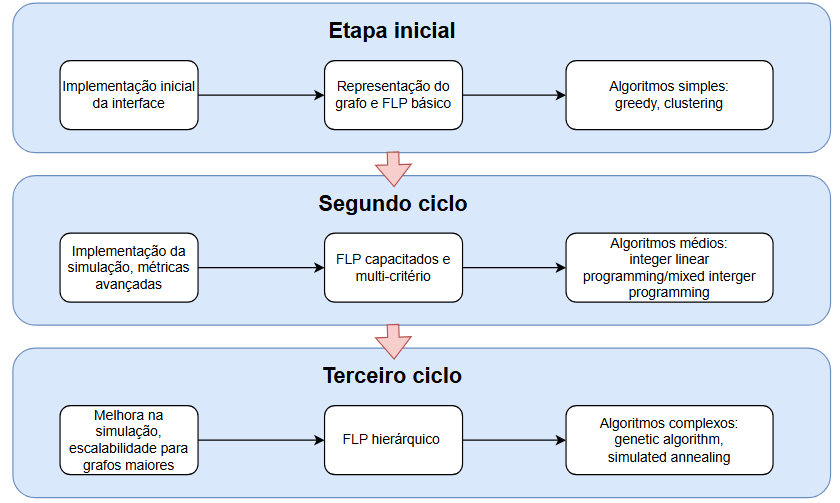
\includegraphics[scale=0.8]{imagens/ciclo_dev.png}
	\end{center}
	\legend{Fonte: Elaboração própria.}
\end{figure}

\FloatBarrier

É importante ressaltar que o ambiente de experimentação desenvolvido não possui caráter educacional. Seu objetivo não é o de ensinar conceitos relacionados a FLP e algoritmos correlatos, mas sim disponibilizar a pesquisadores, profissionais, estudantes e usuários familiarizados com o tema uma ferramenta prática para simulação. A aplicação contará com recursos para ajudar o processo de experimentação, acompanhado por um guia de utilização que orientará o usuário quanto às funcionalidades do programa e ao seu correto manuseio.

Assim como ocorre em problemas de otimização combinatória, a adoção de abordagens exploratórias nem sempre garante a obtenção da solução ótima. O desenvolvimento deste projeto por meio de múltiplas experimentações pode acarretar riscos e desafios, como tempo de execução elevado, dificuldades de escalonamento e eventuais problemas arquiteturais. Entretanto, é importante destacar que a aplicação não tem como objetivo inovar ou resolver todos os problemas do domínio, funcionando apenas como um ambiente de implementação de técnicas já conhecidas. Limitações inerentes a essas técnicas estarão refletidas na aplicação, sendo responsabilidade do usuário compreender essas restrições. Caso algum método se mostre inviável, sua substituição é facilitada pela ampla disponibilidade de alternativas e recursos na literatura, permitindo a adaptação e continuidade do estudo de forma flexível e controlada. 


\section{Aplicação}

\subsection{Modelagem do problema}
Esta seção visa descrever como os dados, como por exemplo o grafo, e os problemas estão estruturados no algoritmo. Poderão ser utilizados trechos de códigos ou diagramas UML para facilitar a visualização da representação.


\subsection{Algoritmos e critérios utilizados}
É fundamental destacar que, em virtude do caráter genérico da aplicação proposta, torna-se necessário avaliar diferentes critérios e algoritmos de forma conjunta, de modo a identificar aqueles que apresentam maior adequação ao domínio em questão. A utilização de certas técnicas depende das propriedades estruturais e matemáticas do problema tratado. Por exemplo, um algoritmo baseado em agrupamento contínuo não pode ser aplicado diretamente sobre um grafo cuja natureza é intrinsecamente discreta. Sendo assim, os algoritmos e critérios utilizados serão definidos e implementados ao longo do tempo de desenvolvimento do projeto

Ao longo do desenvolvimento do projeto, esta seção será utilizada para descrever os algoritmos e critérios disponíveis na aplicação. 

\subsection{Fluxo de Execução}
O usuário final irá entrar no site a partir de um navegador, na qual terá a opção de importar um grafo a partir de um arquivo ou criar um grafo do zero a partir das ferramentas interativas disponíveis. O usuário poderá criar nós e conectar estes usando arestas, e caso clique em um nó, uma janela mostrando suas propriedades será exibida e nela o usuário poderá editar configurações sobre o nó, como marcar ele como um produtor ou consumidor, definir o peso da conexão com outras arestas, definir algumas propriedades relacionadas ao FLP como custo de implementação, entre outras. Tendo seu grafo pronto, o usuário poderá iniciar uma simulação, na qual será responsável por estruturar como será o problema de localização, isto é definir os critérios e o algoritmo a serem utilizados. Ao terminar a simulação, será exibido os resultados obtidos para o usuário, dando a possibilidade de ele salvar estas informações. É importante lembrar que como um dos focos é comparação e otimização, o usuário pode definir diversas estruturas para o problema, selecionando conjuntos de critérios diferentes ou algoritmos diferentes para gerar todos os resultados de uma única vez.

Esta seção será posteriormente populada com várias imagens demonstrando um fluxo de uso padrão da aplicação, detalhando mais como os processos descritos acimas ocorrem de fato.

\section{Arquitetura}

\subsection{Servidor}
O back-end do programa será implementado utilizando o \textit{Spring Framework}, um conjunto de ferramentas para desenvolvimento de aplicações Java que facilita a criação de sistemas robustos e escaláveis, com ênfase nos módulos \textit{Spring Boot}, que permite configurações e inicialização rápida da aplicação, garantindo deploy eficiente, e \textit{Spring Web}, que fornece suporte ao gerenciamento de requisições HTTP, garantindo comunicação eficiente entre o servidor e a interface do usuário. Essa escolha permite a construção de um back-end escalável, modular e de fácil manutenção, adequado à natureza genérica e experimental do ambiente proposto, sendo que a ampla utilização do Spring em projetos e sua performance superior em comparação com outros \textit{frameworks} e bibliotecas que realizam funções similares reforçam sua adequação \cite{springboot-why}.

A linguagem utilizada, como mencionado anteriormente, será Java, cuja natureza orientada a objetos facilita a modelagem de relações hierárquicas, a definição de contratos entre estruturas e a reutilização de código por meio de herança e polimorfismo.

\subsection{Cliente}
A interface do programa será implementada utilizando o \textit{framework React.js}, que se destaca por permitir o desenvolvimento de aplicações \textit{Single Page Application} (SPA) de forma modular, por meio da reutilização de componentes. Essa abordagem torna o código mais organizado, facilita a manutenção e possibilita a criação de interfaces interativas e responsivas. O React também oferece atualização eficiente do DOM por meio do Virtual DOM, garantindo desempenho elevado mesmo em aplicações com grande quantidade de elementos gráficos. 

Uma das principais vantagens do React, é a utilização de uma linguagem \textit{JavaScript XML} (JSX) que  é uma extensão da linguagem JavaScript que permite escrever sintaxe parecida com HTML dentro do código, de forma a escrever componentes de forma facilitada. Para aproveitar os benefícios da tipagem forte, será usada a variante \textit{TypeScript XML} (TSX). Como o navegador padrão não consegue interpretar estas linguagens, é necessário passar por um processo de compilação convertendo estas linguagens para JavaScript puro. Para isso será utilizado o \textit{build tool Vite} que automatiza e otimiza todo o processo, incluindo a transformação de TSX em JavaScript, gerenciamento de módulos e atualização instantânea da interface durante o desenvolvimento.

A renderização dos grafos será realizada utilizando componentes \textit{Scalable Vector Graphics} (SVG), que criam elementos diretamente no DOM do navegador, facilitando a interação e a manipulação individual dos objetos. Diferentemente da renderização baseada em \textit{canvas}, que utiliza uma abordagem de \textit{bitmap}, uma matriz de pixels coloridos, o SVG mantém o conhecimento do navegador sobre cada componente, permitindo atualizações e interações mais simples. Embora a renderização em \textit{canvas} possa ser mais rápida, já que não precisa atualizar o DOM, ela exige que o desenvolvedor implemente grande parte da lógica de interação manualmente, o que aumenta a complexidade do código. Em sistemas com grande número de elementos gráficos, técnicas de renderização baseadas em \textit{bitmap}, como \textit{WebGL}, que aproveita a GPU para cálculos, tendem a apresentar melhor desempenho. Uma abordagem híbrida, que combina diferentes técnicas de renderização de acordo com o nível de zoom ou complexidade dos dados, é ideal em cenários onde o volume de informações pode variar entre simples e complexo.

\subsection{Serviços}
Conforme o desenvolvimento do programa, é possível a necessidade de implementar serviços para lidar com algoritmos complexos ou até mesmo garantir modularização de algum componente da aplicação. Um exemplo de serviço possível é uma API em linguagem Python que recebe dados do Servidor e utiliza-os 
para análises estatísticas ou computação de algum algoritmo. Os serviços implementados serão descritos nessa seção, dando ênfase no tipo de entrada e saída, bem como processamento interno.
%\chapter{Resultados}

Para todos os cenários, foi utilizado um total de 100.000 \texttt{timesteps} que representa
a quantidade de iterações totais que serão feitas. Dentro de um episódio, foi definido
uma taxa de mudanças que o agente pode fazer que influencia no número máximo de mudanças
que é calculado pela taxa multiplicado pelo total de células. Além disso, também é calculado um número máximo de 
iterações que pela multiplicação do número máximo de mudanças pela
quantidade de células totais no labirinto. No caso do experimento, uma taxa de mudança fixa
para os experimentos inicias de 0.3 foi definida, resultando em um máximo de 7 mudanças no
labirinto e um total máximo de 252 iterações. É importante ressaltar que um episódio pode não
realizar todas as iterações, e terminar porque atingiu o máximo de mudanças ou
por uma condição de término de episódio por convergência.


\section{Cenário 1}
Neste primeiro cenário testado, o estado inicial do ambiente é sempre o mesmo para 
todos os episódios, sendo representado por um tabuleiro com todas as células vazias,
exceto pela primeira posição, \([0,0]\), que representa o início, e pela última
posição, \([5,5]\) que representa o objetivo. Esse cenário pode ser observado 
pela Figura \ref{c1}

\begin{figure}[htb]
	\caption{\label{c1}Observação inicial fixa do primeiro cenário}
	\begin{center}
	    \includegraphics[scale=0.5]{imagens/c1.png}
	\end{center}
	\legend{Fonte: Elaboração própria.}
\end{figure}

\FloatBarrier

Esse cenário apresenta uma possível limitação: como os estados iniciais são sempre os mesmos, 
o agente não é exposto a uma diversidade de situações durante o processo de aprendizado. 
Como consequência, ele tende a memorizar uma solução específica para o problema em vez de aprender uma 
política generalizável. Isso implica que, ao ser inserido em um novo cenário, o agente provavelmente 
não conseguirá adaptar-se ou convergir para uma solução adequada, comprometendo sua capacidade de generalização.

No entanto, esse tipo de configuração controlada pode ser útil em etapas iniciais de experimentação, 
pois permite observar com mais clareza o comportamento do modelo e o impacto dos parâmetros sobre os resultados. 
Em ambientes restritos, é possível realizar análises mais precisas e isolar variáveis, o que contribui para a compreensão 
mais profunda do funcionamento do algoritmo antes de aplicá-lo a situações mais complexas e variáveis.


Nesse cenário, o primeiro teste, considerado o mais simples de todos, é que o agente 
consiga criar um labirinto com um tamanho total de 11 células. Neste caso, o labirinto já
vem pré-definido com uma distância de 10 células entre o início e o final, então o agente,
em teoria, não precisa modificar muito o cenário. Nesse caso, o agente só pode colocar 
células vazias ou paredes, e sua função de recompensa é parametrizada pelo tamanho 
do caminho entre o início e o fim, sendo utilizado a função de recompensa que compara
a diferença entre dois estados.

\begin{figure}[htb]
	\caption{\label{mr_c1r3}Recompensa média ao longo do treino por representação}
	\begin{center}
	    \includegraphics[scale=0.5]{imagens/mr_c1r3.png}
	\end{center}
	\legend{Fonte: Elaboração própria.}
\end{figure}

\begin{figure}[htb]
	\caption{\label{el_c1r3}Tamanho total de episódios por representação}
	\begin{center}
	    \includegraphics[scale=0.5]{imagens/el_c1r3.png}
	\end{center}
	\legend{Fonte: Elaboração própria.}
\end{figure}

\FloatBarrier

Como é possível observar pelas Figuras \ref{mr_c1r3} e \ref{el_c1r3}, todas as representações tendem a seguir o mesmo comportamento,
com \textit{Wide} tendo um crescimento ao longo do tempo e obtendo, no final, o melhor valor. Entretanto, a
representação \textit{Narrow Fixed} tem um comportamento bastante caótico e tem alta variância. Este tipo de
comportamento é relativamente esperado já que a representação sempre terá um padrão de observação fixo. Isto 
misturado com o fato de que o estado inicial sempre é fixo faz com que o modelo nunca realmente aprenda nada.
A Figura \ref{c1-nf} mostra o labirinto final gerado por esta representação

\begin{figure}[htb]
	\caption{\label{c1-nf}Estado final da representação \textit{Narrow Fixed}}
	\begin{center}
	    \includegraphics[scale=0.5]{imagens/c1-nfr3.png}
	\end{center}
	\legend{Fonte: Elaboração própria.}
\end{figure}

\FloatBarrier

Como é possível perceber, como a representação sempre começa pela primeira posição e percorre o ambiente de forma sequencial, 
ela tende a focar nas regiões iniciais do labirinto e a desprezar completamente o restante do espaço. 
Isso ocorre porque o agente, ao explorar e atribuir valores aos estados, atualiza prioritariamente as 
primeiras células que encontra, e raramente alcança ou dá atenção às partes mais distantes.



Este comportamento acaba criando um viés espacial muito forte, onde os estados iniciais são 
atualizados com frequência enquanto os estados mais distantes permanecem praticamente inalterados. 
Isso pode ser observado claramente pela Figura \ref{c1-nf}: as células localizadas na primeira e segunda fileiras 
tiveram seus valores significativamente modificados, enquanto o restante do labirinto manteve-se  
inalterado, como se fosse invisível para o agente.

Tal limitação compromete a generalização da política aprendida, uma vez que o agente se torna 
especializado em uma região muito restrita do ambiente. Além disso, esse tipo de representação 
impede uma exploração eficaz e dificulta a aprendizagem de trajetórias que envolvem 
regiões mais profundas e complexas do labirinto.

Diante desses problemas, essa abordagem de representação não é adequada para este tipo de ambiente. 
Por isso, a partir deste ponto, foi optado por não utilizar mais essa representação nas próximas análises e experimentos. 



Após estes testes, foi feito outro muito parecido, mas considerando um novo 
parâmetro na recompensa que é o número de paredes. Assim, o agente é estimulado 
a inserir paredes, de certa forma o guiando para maximizar a verdadeira função objetivo
que é aumentar o caminho entre o início e o objetivo

\begin{figure}[htb]
	\caption{\label{mr_c1r3_1}Recompensa média ao longo do treino por representação, considerando a quantidade de paredes}
	\begin{center}
	    \includegraphics[scale=0.5]{imagens/mr_c1r3_1.png}
	\end{center}
	\legend{Fonte: Elaboração própria.}
\end{figure}

\begin{figure}[htb]
	\caption{\label{el_c1r3_1}Tamanho total de episódios por representação, considerando a quantidade de paredes}
	\begin{center}
	    \includegraphics[scale=0.5]{imagens/el_c1r3_1.png}
	\end{center}
	\legend{Fonte: Elaboração própria.}
\end{figure}

\FloatBarrier


Como é possível perceber pelas Figuras \ref{mr_c1r3_1} e \ref{el_c1r3_1}, 
a introdução da nova métrica ajudou bastante na convergência do algoritmo, 
significando que as duas métricas estão complementando uma as outras. 
Também é possível perceber que o número total de episódios aumentou, o que pode ser algo bom, pois mostra que o agente
está interagindo bastante com o ambiente e realizando mudanças ou ele consegue atingir as condições necessárias de término.

Para verificar a fundo, os valores das métricas e as recompensas, foi feito um teste com um total de mil episódios, 
considerando o melhor modelo encontrado no cenário de treino, das representações \textit{Wide} e \textit{Narrow Random}.
Como utilizar o tamanho do caminho em conjunto com o número de paredes obteve o melhor resultado, este cenário foi analisado
em maior profundidade.

Como é possível perceber pelas Figuras \ref{dd_c1r3_1} e \ref{dd_nrc1r3_1}, a representação \textit{Wide} teve sucesso em todos os cenários de treino, algo que parece bom, mas 
na verdade só enfatiza o problema anteriormente mencionado, dessa representação tender a decorar somente um tipo de estado 
possível, já que não existe nenhum fator de aleatoriedade inserido. Já a representação \textit{Narrow Random} obteve uma 
grande variedade de resultados, destacando-o fato de que mesmo possuindo valores de recompensa baixos, ela ainda consegue
criar labirintos e não tende a produzir unicamente estados impossíveis.

\begin{figure}[htb]
	\caption{\label{dd_c1r3_1}Distribuição de variáveis da representação \textit{Wide}}
	\begin{center}
	    \includegraphics[scale=0.5]{imagens/dd_c1r3_1.png}
	\end{center}
	\legend{Fonte: Elaboração própria.}
\end{figure}

\begin{figure}[htb]
	\caption{\label{dd_nrc1r3_1}Distribuição de variáveis da representação \textit{Narrow Random}}
	\begin{center}
	    \includegraphics[scale=0.5]{imagens/dd_nrc1r3_1.png}
	\end{center}
	\legend{Fonte: Elaboração própria.}
\end{figure}

\FloatBarrier



A Figura \ref{c1_end} apresenta um exemplo de estado final de um episódio das duas representações \textit{Narrow Random} e \textit{Wide},
considerando os dois exemplos: com o caminho entre início e fim considerado isoladamente e 
considerado este em conjunto com a métrica de quantidade de paredes.
\begin{figure}[htb]
	\caption{\label{c1_end}Exemplos de estados finais}
	\begin{center}
	    \includegraphics[scale=0.5]{imagens/c1-end.png}
	\end{center}
	\legend{Fonte: Elaboração própria.}
\end{figure}

\FloatBarrier
É importante ressaltar que como \textit{Wide} tem sempre controle total das posições, ele vai aprender a decorar um padrão, pois o estado
inicial é sempre o mesmo, um comportamento que não ocorre quando se considera \textit{Narrow Random}, já que apesar de o estado inicial 
nunca mudar, a representação sempre está vendo um conjunto de células diferentes em cada episódio. Isso demonstra a importância de 
sempre considerar um grau de aleatoriedade na estruturação do problema, mesmo se for no estado inicial ou nas representações
de espaço de ação do agente gerador.



\section{Cenário 2}
Este cenário, possui as mesmas características do anterior, só que agora o objetivo é testar
um estado inicial aleatório, sempre com uma posição inicial e uma final. Uma imagem de uma geração
possível pode ser visualizada pela Figura \ref{c2}

\begin{figure}[htb]
	\caption{\label{c2}Representação de um cenário inicial aleatório}
	\begin{center}
	    \includegraphics[scale=0.5]{imagens/c2.png}
	\end{center}
	\legend{Fonte: Elaboração própria.}
\end{figure}

\FloatBarrier

As mesmas métricas do cenário anterior foram testadas, primeiramente utilizando o \textit{path\_length} sozinho e depois
em conjunto com \textit{num\_wall}. O resultado do primeiro experimento pode ser observado pelas Figuras \ref{mr_c2r3}
e \ref{el_c2r3}.

\begin{figure}[htb]
	\caption{\label{mr_c2r3}Recompensa média ao longo do tempo por representação}
	\begin{center}
	    \includegraphics[scale=0.5]{imagens/mr_c2r3.png}
	\end{center}
	\legend{Fonte: Elaboração própria.}
\end{figure}

\begin{figure}[htb]
	\caption{\label{el_c2r3}Tamanho total de episódios por representação}
	\begin{center}
	    \includegraphics[scale=0.5]{imagens/el_c2r3.png}
	\end{center}
	\legend{Fonte: Elaboração própria.}
\end{figure}

\FloatBarrier

O algoritmo apresenta um comportamento semelhante ao apresentado no cenário anterior em questão de convergência e valores
obtidos de retorno. Isso mostra que mesmo introduzindo aleatoriedade, a representação \textit{Wide} conseguiu se adaptar
bem e produzir bons resultados.


O teste com as duas métricas em conjunto pode ser visualizado nas Figuras 
\ref{mr_c2r3_1} e \ref{el_c2r3_1}, que mostram, respectivamente, a 
recompensa média ao longo do tempo e o tamanho total de episódios por representação.
\begin{figure}[htb]
	\caption{\label{mr_c2r3_1}Recompensa média ao longo do tempo por representação}
	\begin{center}
	    \includegraphics[scale=0.5]{imagens/mr_c2r3_1.png}
	\end{center}
	\legend{Fonte: Elaboração própria.}
\end{figure}

\begin{figure}[htb]
	\caption{\label{el_c2r3_1}Tamanho total de episódios por representação}
	\begin{center}
	    \includegraphics[scale=0.5]{imagens/el_c2r3_1.png}
	\end{center}
	\legend{Fonte: Elaboração própria.}
\end{figure}

\FloatBarrier

Pela análise destes gráficos, é possível observar que a 
introdução de uma métrica nova, também auxiliou no cenário 
onde todos os estados iniciais são gerados aleatoriamente. Para analisar as métricas, foram testados mil épocas da
representação \textit{Wide} com os valores de recompensa considerando as duas métricas.

\begin{figure}[htb]
	\caption{\label{dd_wrc2r3_1}Distribuição de variáveis da representação Wide}
	\begin{center}
	    \includegraphics[scale=0.5]{imagens/dd_wrc2r3_1.png}
	\end{center}
	\legend{Fonte: Elaboração própria.}
\end{figure}

\FloatBarrier

Como é possível observar pela Figura \ref{dd_wrc2r3_1}, aconteceu um fenômeno diferente dos observados até agora: 
a grande maioria dos episódios
atingiu o término pelo limite máximo de iterações possíveis.
Isso significa que o agente não está mais realizando mudanças no ambiente, 
o que pode indicar um problema clássico de exploração versus explotação. 
Nesse cenário, o agente pode ter adotado uma política subótima, levando-o a estagnar em um comportamento pouco eficiente. 
Além disso, é possível que ele tenha aprendido que realizar muitas mudanças tende a resultar em recompensas menores, 
o que o leva a preferir não agir e, assim, evitar penalidades.

É importante considerar que um agente não alterar o estados de um labirinto entre 
duas iterações pode ser algo ruim. Se não houver nenhum custo para ficar 
parado ou inalterado, e as mudanças tendem a penalizar ou não recompensar o agente, 
o caminho de menor resistência é não fazer nada. Isso gera uma estagnação, e uma 
convergência. Quando o gerador aprende a não mudar nada para minimizar consequências 
negativas, ele está basicamente "jogando seguro" — o que é um comportamento comum em 
RL quando a função de recompensa não incentiva exploração ou mudança. 


Apesar disso, é possível observar que só em torno de 13,7\% dos casos o agente acaba modificando o labirinto
e tornando-o inviável. O comportamento observado aqui exemplifica que só se basear em funções de valor para
estimar a performance de um modelo não é algo desejável, já que o agente pode ter internalizado uma política
sub-ótima que dificultaria sua performance em generalizações.

A Figura \ref{c2-end} apresenta um exemplo de estado final de um episódio das duas representações 
\textit{Narrow Random} e \textit{Wide},
considerando os dois exemplos: com o caminho entre início e fim considerado isoladamente e 
considerado este em conjunto com a métrica de quantidade de paredes.

\begin{figure}[htb]
	\caption{\label{c2-end}Exemplos de estados finais}
	\begin{center}
	    \includegraphics[scale=0.8]{imagens/c2-end.png}
	\end{center}
	\legend{Fonte: Elaboração própria.}
\end{figure}

\FloatBarrier

Foram considerados várias amostras da representação \textit{Wide} mas foi percebido que elas tendem a realizar poucas ações
no ambiente e depois congelam. Além disso, as ações que realizam parecem não representar mudanças muito efetivas, no
contexto da criação e execução da fase. Em contrapartida, a representação \textit{Narrow Random} parece capturar muito bem
uma tendência em mudar células em torno do início ou objetivo, de forma a tornar o caminho mais comprido. O gráfico abaixo
foi feito para comparar os tamanhos de caminhos, entre as duas representações, sendo a \textit{Narrow Random} considerado
as duas possíveis recompensas.

\begin{figure}[htb]
	\caption{\label{dd_nrc2}Distribuição de \textit{path\_length} na \textit{Narrow Random}}
	\begin{center}
	    \includegraphics[scale=0.5]{imagens/dd_nrc2.png}
	\end{center}
	\legend{Fonte: Elaboração própria}
\end{figure}

\FloatBarrier
Com a análise da Figura \ref{dd_nrc2}, é perceptível que, apesar das diferenças notáveis do ponto de vista visual, a comparação 
entre as distribuições de caminhos geradas por ambas as representações revela uma 
variação pouco significativa em termos quantitativos. Esse resultado evidencia uma 
das principais dificuldades enfrentadas no uso de aprendizado por reforço no contexto 
da geração procedural de conteúdo: a complexidade de se modelar, de forma computacional, 
percepções humanas subjetivas. Em outras palavras, nem sempre é trivial traduzir elementos 
visuais, estéticos ou emocionais, inerentemente humanos, em representações que possam ser 
compreendidas e abstraídas por um agente gerador. Essa limitação ressalta o desafio de alinhar 
métricas computacionais com interpretações qualitativas sutis e dependentes de um maior contexto.



\section{Cenário 3}
Neste cenário, uma geração aleatória é utilizada baseada na seguinte probabilidade:
\begin{itemize}
    \item Célula vazia: 70\%;
    \item Célula de parede: 20\%;
    \item Célula de início: 5\%;
    \item Célula de fim: 5\%.
\end{itemize}
A distribuição de probabilidades visa, portanto, equilibrar explorabilidade e complexidade: 
uma grande quantidade de células vazias facilita a navegação do agente nos estágios iniciais do aprendizado,
enquanto uma porcentagem controlada de paredes introduz obstáculos e variações estruturais que promovem a generalização da política.
Se fosse definido uma geração totalmente aleatória, o algoritmo demoraria muito para convergir, pois teria que lidar com muitos
cenários que não fazem sentindo, podendo até mesmo prejudicar no seu aprendizado. Um exemplo de cenário pode ser visualizado pela
Figura \ref{c3}:

\begin{figure}[htb]
	\caption{\label{c3}Representação de um cenário inicial aleatório}
	\begin{center}
	    \includegraphics[scale=0.5]{imagens/c3.png}
	\end{center}
	\legend{Fonte: Elaboração própria}
\end{figure}

\FloatBarrier

O primeiro teste nesse ambiente foi considerando que o agente pode apenas alterar células do tipo de início e fim.
O objetivo disso é fazer com que o agente aprende a balancear um ambiente caótico e impossível de ser resolvido 
em um ambiente estável. Nos testes anteriores, o agente demonstrou certa aprendizado em não alterar células de 
início e fim, e só mudar paredes, já que esse comportamento gera uma recompensa. Porém o cenário descrito é simples,
com apenas uma célula de classes não predominantes, então no cenário randômico, a intenção é o agente aprender 
a lidar com um número de parâmetros variáveis. Para realização deste teste, é utilizado uma função que compara 
valores antigos com os novos, e recompensa um total de células de tipo início e fim que se aproxima de um.
As Figuras \ref{s_cr} e \ref{e_cr} apresentam a comparação da distribuição de células de início e fim entre as duas
representações.

\begin{figure}[htb]
	\caption{\label{s_cr}Distribuição de células do tipo \textit{start} nas representações }
	\begin{center}
	    \includegraphics[scale=0.5]{imagens/s_cr.png}
	\end{center}
	\legend{Fonte: Elaboração própria}
\end{figure}

\begin{figure}[htb]
	\caption{\label{e_cr}Distribuição de células do tipo \textit{end} nas representações }
	\begin{center}
	    \includegraphics[scale=0.5]{imagens/e_cr.png}
	\end{center}
	\legend{Fonte: Elaboração própria}
\end{figure}


\FloatBarrier

Como é possível perceber, pela análise das Figuras \ref{s_cr} e \ref{e_cr}, a representação \textit{Narrow Random} apresenta um resultado
muito ruim quando considerados as células de início, com variações muito altas que fogem do valor otimizado. A outra
representação possui valores menos variados, mas ainda assim, não tem uma performance considerada satisfatória. 

Um gráfico para analisar as recompensas no treino pode ser observado abaixo, 
permitindo uma visão mais clara do comportamento do agente ao longo dos episódios e de 
como ele responde às recompensas atribuídas pelo ambiente. 
\begin{figure}[htb]
	\caption{\label{se}Recompensas médias ao longo do tempo nas duas representações}
	\begin{center}
	    \includegraphics[scale=0.5]{imagens/se.png}
	\end{center}
	\legend{Fonte: Elaboração própria}
\end{figure}

\FloatBarrier

Analisando a Figura \ref{se}, observa-se um comportamento inesperado em relação ao que havia sido identificado 
anteriormente: a representação \textit{Narrow Random} apresentou resultados superiores, 
com recompensas médias mais elevadas. Isso contrasta com o desempenho ruim anteriormente observado, 
especialmente no que diz respeito às células de início, onde apresentava grande variação e distanciamento 
dos valores ideais. Esse contraste sugere que, apesar de suas limitações em aspectos estruturais específicos, 
a \textit{Narrow Random} pode favorecer uma maior diversidade de trajetórias e estratégias, 
resultando em melhores recompensas acumuladas ao longo do tempo em determinados contextos.

Isso evidencia um dos principais desafios no contexto de PCG, na qual as funções de recompensa nem sempre são facilmente interpretáveis. 
Embora a análise visual do layout do labirinto permita uma compreensão mais intuitiva do comportamento do modelo, 
a avaliação baseada exclusivamente em métricas estatísticas pode levar a interpretações equivocadas. 
Essa discrepância ressalta a importância de combinar abordagens quantitativas e qualitativas na 
análise do desempenho de agentes em ambientes gerados proceduralmente.


O segundo teste neste cenário, é testar um cenário complexo, no qual o agente pode alterar todos os tipos de células, tendo 
o máximo de controle possível sobre o ambiente. Nesse exemplo, foram considerados como métricas importantes o tamanho do caminho
do início até o fím, o número de paredes, de células de início e de fim. O peso das paredes foi definido para tres para
tentar auxiliar na convergência do agente. Os dados de treino, podem ser visualizados abaixo:

\begin{figure}[htb]
	\caption{\label{scenario4}Recompensas médias ao longo do tempo nas duas representações}
	\begin{center}
	    \includegraphics[scale=0.5]{imagens/scenario4.png}
	\end{center}
	\legend{Fonte: Elaboração própria}
\end{figure}

\FloatBarrier

Pela análise da Figura \ref{scenario4}, tem se a impressão de que o algoritmo esta convergindo, pois a recompensa esta aumentando a medida do
tempo e se estabilizando em valores não tão distantes em relação aos observados anteriormente. Porém, ao analisar mais a fundo, com
o treinamento do melhor modelo encontrado, foi descoberto um comportamento longe do ideal

\begin{figure}[htb]
	\caption{\label{r4_pl}Distribuição do tamanho do caminho nas duas representações}
	\begin{center}
	    \includegraphics[scale=0.5]{imagens/r4_pl.png}
	\end{center}
	\legend{Fonte: Elaboração própria}
\end{figure}

\FloatBarrier

Como é possível perceber pela Figura \ref{r4_pl}, mais de 90\% dos labirintos gerados são considerados inválidos. Isso ressalta outro 
problema de depender somente da análise das recompensas ao longo do tempo, pois mesmo que o agente pareça convergir, ele pode, 
na verdade, estar apresentando um comportamento muito ruim. O principal motivo pela função de recompensa apresentar valores, que 
podem não ser considerados ruins de primeira vista, é a grande complexidade que é gerada ao usar de um ambiente com muitas variáveis.
Quanto mais se adiciona variáveis, maior a chance de elas acabarem tendo uma certa dependência e correlação entre si, tornando o processo
de modelagem de função de recompensa algo muito complexo que raramente irá representar resultados ótimos. A Figura \ref{r4_nwall} 
está representando a distribuição de \texttt{path\_length}.

\begin{figure}[htb]
	\caption{\label{r4_nwall}Distribuição do número de paredes nas duas representações}
	\begin{center}
	    \includegraphics[scale=0.5]{imagens/r4_nwall.png}
	\end{center}
	\legend{Fonte: Elaboração própria}
\end{figure}

\FloatBarrier

Como é de se esperar, a função apresenta uma distribuição gaussiana dos valores de paredes, pois foi definido um peso priorizando elas.
Muito provavelmente, a função aprendeu a colocar paredes para obter melhores recompensa, e não está se importando em arrumar a quantidade
de células de início e fim, já que irão garantir menos recompensa. Entretanto, manter todas as células com o mesmo peso, faz com que o modelo
não saiba para qual métrica dar mais "atenção", resultando em um modelo que converge muito mais lento pois precisará explorar muito mais.
Foi feito um teste para avaliar o impacto em equalizar o peso entre todas as métricas:

\begin{figure}[htb]
	\caption{\label{r5-X}Recompensas médias ao longo do tempo}
	\begin{center}
	    \includegraphics[scale=0.5]{imagens/r5-X.png}
	\end{center}
	\legend{Fonte: Elaboração própria}
\end{figure}

\begin{figure}[htb]
	\caption{\label{w5-x}Distribuição de métricas ao equalizar os pesos}
	\begin{center}
	    \includegraphics[scale=0.5]{imagens/w5-x.png}
	\end{center}
	\legend{Fonte: Elaboração própria}
\end{figure}

\FloatBarrier
Comparando os resultados observados nas Figuras \ref{r5-X} e \ref{w5-x}, 
deixar todos os pesos iguais não surtiu em nenhum efeito, considerando 
a o número de caminhos inválidos gerados e a distribuição do número de paredes. Isso exemplifica um dos grandes
problemas relacionados a utilização de recompensas ponderas, já que é difícil estimar um valor que tenha impacto 
o suficiente, sem atrapalhar na convergência e resultados finais do gerador. Além disso, a escolha de qual 
métrica utilizar na ponderação, pode não ser clara, dependendo de vários testes extensivos para estimação de comportamento,
já que as variáveis de um problema podem ter comportamentos exclusivos ou inclusivos e o gerador pode interpretar
esses comportamentos de maneira não padronizada.


\section{Taxa de mudança}
Para testar a influência da taxa de mudança, que controla o quanto o agente pode mudar o ambiente, foi utilizado o "cenário 2" e 
a representação do tipo \textit{Narrow Random} com duas métricas de recompensa, por obter bons resultados nos experimentos realizados.
Como todos os experimentos foram realizadas com uma taxa relativamente baixa de 0.3, será 
proposto a utilização de um valor muito baixo de 0.1, um valor intermediário de 0.5 e um valor alto 
de 1 que simboliza o maior tipo de mudança. A Figura \ref{change_rate} mostra a recompensa média por tempo em relação a taxa de mudança
selecionada.

\begin{figure}[htb]
	\caption{\label{change_rate}Recompensas médias ao longo do tempo}
	\begin{center}
	    \includegraphics[scale=0.5]{imagens/change_rate.png}
	\end{center}
	\legend{Fonte: Elaboração própria}
\end{figure}

\FloatBarrier

O gráfico acima ilustra muito bem, como é importante considerar de maneira cuidadosa os valores de taxa de mudança que um agente 
pode realizar em um ambiente. Valores altos, fazem com que o agente sempre queira ficar alterando algo, fazendo com que o 
espaço de observações seja transformado muitas vezes durante o episódio, causando instabilidade nas recompensas e 
dificuldade na convergência. Isto é
exemplificado no gráfico, onde inicialmente existe um leve crescimento, mas o algoritmo começa a performar mal e 
seu desempenho cai, algo muito raro de acontecer, já que geralmente o agente converge para um valor, mesmo que não seja
o ótimo. Já uma taxa de mudança baixa obteve um ótimo desempenho com valores convergindo para o melhor cenário possível,
mostrando que nesse cenário, quanto mais o agente muda o ambiente, pior serão as recompensas obtidas. É importante ressaltar
que essa mudança vária de acordo com a complexidade do caso que está sendo analisado, já que, em jogos mais complexos, pode
ser necessário um maior conjunto de ações para alcançar um estado desejável. A Figura \ref{cr01metrics} analisa em
maior detalhe algumas métricas de desempenho considerando uma taxa de mudança de 0.1.
\begin{figure}[htb]
	\caption{\label{cr01metrics}Métricas avaliadas do modelo com taxa de mudança de 0.1}
	\begin{center}
	    \includegraphics[scale=0.5]{imagens/cr01metrics.png}
	\end{center}
	\legend{Fonte: Elaboração própria}
\end{figure}

\FloatBarrier
Como é possível observar pela figura acima, nem sempre um modelo que está convergindo para valores
muito próximos de zero terá um resultado ótimo. Apesar de o agente conseguir criar, na grande maioria dos casos, 
caminhos viáveis no labirinto, ele sempre está realizando três ações, que é o total possível nesse cenário. Esse fato,
mostra que a taxa escolhida poderia ser um pouco melhor, pois pelo fato de o agente sempre escolher realizar o mesmo
número máximo de ações significa que ele "enxerga"\ estas ações como valiosas e impactantes para maximizar a recompensa,
então realizar mais ações provavelmente traria ainda mais valores de retorno positivo.









\section{Problemas encontrados}

\subsection{Recompensa}
Durante o desenvolvimento e a realização dos testes, foi possível observar que a definição das funções de recompensa 
representa um dos aspectos mais sensíveis e desafiadores do processo de aprendizado por reforço. 
Em ambientes de geração procedural, por exemplo, a construção de recompensas baseadas apenas em uma métrica isolada, 
como o comprimento do caminho em um labirinto, pode se mostrar ineficaz. Embora tal métrica possa, em tese, 
incentivar o agente a produzir mapas mais interessantes ou desafiadores, ela não é suficiente para capturar 
a complexidade do cenário. Isso ocorre porque o comprimento do caminho é, frequentemente, influenciado por 
outras variáveis estruturais, como o número e a posição das paredes. Assim, o agente pode acabar otimizando 
aspectos colaterais que não representam diretamente o objetivo desejado, dificultando a convergência e levando 
a comportamentos sub-ótimos.

Por outro lado, incluir múltiplos componentes de recompensa, como a quantidade de células de início e fim, 
também apresenta desafios. Quando muitas recompensas são combinadas, o agente pode ter dificuldade em determinar 
quais delas deve priorizar, levando a um aprendizado ambíguo ou até mesmo contraditório. Isso pode 
obfuscar o verdadeiro objetivo do ambiente, impedindo que o comportamento aprendido seja consistente ou generalizável.

Adicionalmente, recompensas mal definidas ou fortemente correlacionadas (i.e., variáveis dependentes) 
podem interferir negativamente no aprendizado, já que modificações em uma métrica podem afetar inadvertidamente outras. 
Esse tipo de sobreposição pode levar o agente a interpretar sinais de maneira errada, ou explorar caminhos de otimização não intencionais.



Outro ponto crítico é a definição dos pesos associados a cada componente da função de recompensa. 
Ajustar esses pesos é uma tarefa não trivial e, muitas vezes, altamente empírica. Pequenas variações 
podem induzir prioridades indesejadas, fazendo com que o agente desenvolva comportamentos que maximizam 
recompensas irrelevantes ou até prejudiciais à qualidade do mapa gerado. Em ambientes complexos e 
com múltiplos objetivos, encontrar uma combinação de pesos que represente fielmente as intenções 
do projetista do ambiente é um grande desafio, frequentemente exigindo muitas iterações e testes manuais.



Esses desafios na definição e balanceamento das funções de recompensa evidenciam que a aplicação de 
algoritmos de Reinforcement Learning para tarefas de geração procedural de conteúdo pode não ser, necessariamente, 
a abordagem mais prática ou eficiente no contexto do desenvolvimento de jogos. Isso se deve ao fato de que esses ambientes 
exigem um grau elevado de precisão na formulação do problema e um entendimento aprofundado sobre a influência de múltiplas 
variáveis no comportamento do agente. No entanto, na prática, desenvolvedores de jogos nem sempre dispõem do conhecimento 
técnico necessário para elaborar funções de recompensa bem calibradas ou formalizar com clareza os objetivos desejados em termos 
computacionais.

Consequentemente, mesmo que um determinado algoritmo de RL demonstre excelente desempenho em estudos acadêmicos ou benchmarks controlados, 
sua replicação por profissionais da indústria pode se mostrar limitada. Isso ocorre não por deficiência do algoritmo em si, mas 
pela dificuldade prática de traduzir objetivos subjetivos, como jogabilidade, diversão ou desafio, em métricas formais que 
conduzam o agente ao comportamento desejado. Este problema mencionado, tende a se evidenciar ainda mais quanto
maior a complexidade de um jogo, em relação a quantidade de variáveis que uma fase pode conter. Assim, o sucesso 
da aplicação de RL nesse domínio depende não apenas da escolha do 
algoritmo, mas também da capacidade de modelagem do problema, o que pode representar uma barreira significativa fora do 
ambiente de pesquisa.

\subsection{Representação}
Um dos principais desafios enfrentados durante o desenvolvimento deste trabalho foi a representação adequada 
do espaço de estados e ações no contexto da geração procedural de fases. A tarefa de geração de conteúdo em jogos, 
especialmente em ambientes como labirintos ou plataformas, envolve uma grande variedade de elementos e estruturas possíveis. 
Essa diversidade resulta em espaços de ação e observação altamente dimensionais, o que dificulta significativamente o 
processo de aprendizado por reforço.

Como tentativa de mitigar esse problema, foram testadas diferentes formas de modelagem do agente, 
alterando a maneira como ele percebe o ambiente e decide suas ações. No entanto, mesmo com essas adaptações, a 
definição de uma representação que fosse ao mesmo tempo expressiva e eficiente mostrou-se desafiadora. 
A depender da estruturação do problema, é possível criar agentes que demonstram bom desempenho em executar 
determinados tipos de ações ou em operar dentro de padrões específicos do espaço de estados. 
No entanto, ao se empregar múltiplas formas de representação, pode ocorrer sobreposição ou
divergência significativa entre os comportamentos dos agentes. Em alguns casos, diferentes representações 
produzem agentes com métricas e comportamentos muito semelhantes; em outros, os resultados podem variar drasticamente. 
Essa inconsistência dificulta a realização de comparações diretas, comprometendo a análise objetiva sobre a 
eficácia de cada modelagem. Esse cenário evidencia a complexidade envolvida na escolha da representação ideal e 
ressalta a importância de métodos mais padronizados ou de métricas que capturem melhor as nuances entre os diferentes agentes.

Sendo assim, o desalinhamento entre a complexidade do espaço e a capacidade de generalização do agente impacta 
diretamente na qualidade do conteúdo gerado, tornando o processo de treinamento mais demorado e instável. 
Dessa forma, a representação do espaço permanece como um dos principais pontos críticos na aplicação de RL para PCG, 
exigindo abordagens mais sofisticadas e, possivelmente, métodos híbridos que integrem conhecimento prévio ou aprendizado 
supervisionado para guiar o processo de modelagem.

\section{Considerações Finais}
Embora nenhum dos experimentos realizados neste trabalho tenha convergido para uma política ótima que maximize 
consistentemente a recompensa total, isso não invalida o uso de algoritmos de aprendizado por reforço, 
como o Proximal Policy Optimization (PPO), em tarefas de geração procedural de conteúdo em jogos digitais. 
Os resultados obtidos indicam que, mesmo diante da ausência de uma convergência clara, o agente ainda foi 
capaz de produzir conteúdos válidos, neste caso, labirintos jogáveis e estruturalmente coerentes o que 
demonstra a viabilidade de tais abordagens mesmo em cenários de alta complexidade.

É importante destacar que as funções de recompensa utilizadas foram cuidadosamente elaboradas com o 
intuito de induzir o agente a maximizar métricas específicas relacionadas à qualidade do conteúdo gerado. 
Entretanto, a formulação dessas recompensas pode ter limitado a capacidade de generalização e adaptação do agente, 
evidenciando a sensibilidade dos algoritmos de RL à definição dessas funções. Ainda assim, os modelos 
treinados apresentam potencial como geradores pseudoaleatórios, que, embora não alcancem soluções ótimas, 
aprendem a evitar casos extremos ou inválidos ao internalizar parcialmente os critérios estabelecidos pelas 
recompensas durante o processo de otimização.

Outro ponto crítico observado ao longo dos experimentos é a elevada quantidade de hiperparâmetros 
e decisões de modelagem envolvidos na estruturação do problema. Aspectos como o formato do espaço de observação, 
a granularidade das ações, os tipos de cenários utilizados nos testes e a própria taxa de atualização do ambiente 
influenciam diretamente o desempenho e a estabilidade do treinamento. Nesse sentido, a decomposição do 
problema em subcomponentes mais simples, cada um com objetivos mais específicos e mensuráveis,
pode representar uma estratégia eficiente para mitigar a complexidade envolvida.

Além disso, abordagens baseadas em \textit{Meta-Learning}, que visam permitir que o próprio sistema aprenda a 
otimizar seus hiperparâmetros ou estrutura interna, podem desempenhar um papel fundamental na automação e 
aprimoramento desses processos. Tais abordagens não apenas facilitam a adaptação a diferentes domínios, 
como também reduzem o custo cognitivo e computacional associado à experimentação manual intensiva.

Como trabalhos futuros, é recomendável explorar técnicas que reduzam a alta dimensionalidade dos espaços 
de ação e observação, um dos principais desafios enfrentados neste tipo de tarefa. 
Estratégias como a decomposição do processo de geração em subetapas mais simples podem facilitar o 
aprendizado, além de permitir maior controle sobre aspectos específicos do conteúdo gerado. 
A integração de abordagens de \textit{multi-task learning} também se apresenta como uma alternativa promissora, 
possibilitando que o agente aprenda simultaneamente múltiplas habilidades relacionadas à geração de conteúdo. 
Por fim, sugere-se a investigação de algoritmos híbridos que combinem aprendizado por reforço com métodos 
baseados em dados, como \textit{imitation learning} ou \textit{offline RL}, a fim de acelerar a convergência 
e melhorar a qualidade do conteúdo gerado mesmo em contextos com sinais de recompensa esparsos.





%\chapter{Conclusão}
O mercado de jogos vem crescendo cada vez mais e cada vez mais pessoas estão interessadas em participar
dessa nova tendência. O uso de inteligência artificial (IA) no desenvolvimento de jogos digitais tem se 
consolidado como uma ferramenta poderosa para automatizar tarefas complexas, ampliar possibilidades criativas 
e reduzir o custo de produção. Dentre as diversas aplicações possíveis, a geração procedural de conteúdo (PCG) é uma
técnica clássica já bastante implementada, porém vem se reintegrando e modificando-se para adaptar-se aos novos
poderosos algoritmos de IA. A enorme presença de diferentes algoritmos cria um ecossistema de inovação constante,
cada algoritmo com suas vantagens em desvantagens. O aprendizado por reforço representa uma abordagem promissora, 
principalmente por sua capacidade de operar sem dados de treinamento previamente disponíveis, uma limitação comum em jogos
ainda em fase de desenvolvimento. Essa característica torna os métodos baseados em RL particularmente adequados 
para auxiliar diretamente o processo criativo no design de jogos, contribuindo para a geração dinâmica 
e adaptativa de níveis, mapas e outros elementos.

Neste trabalho, foram exploradas diferentes estruturas de modelagem do problema de PCG utilizando RL, investigando o 
impacto de múltiplos fatores: recompensas personalizadas, variações no espaço de estados e ações, cenários com diferentes 
configurações de labirintos e alterações na taxa de atualização do ambiente. As experiências demonstraram que, 
ainda que os algoritmos, em especial o \textit{Proximal Policy Optimization} (PPO), não tenham atingido uma política ótima, 
foi possível observar a capacidade dos modelos em gerar conteúdos válidos e coerentes. 
Isso indica que, mesmo sem convergir completamente, os agentes aprendem a evitar soluções inviáveis e a respeitar certas 
restrições estruturais implícitas no ambiente.

A análise dos resultados revelou também alguns dos principais desafios enfrentados ao aplicar RL no contexto de PCG, 
como o alto custo computacional, a sensibilidade à definição das recompensas e a complexidade de se trabalhar com espaços de ação e 
observação de alta dimensionalidade. Tais dificuldades reforçam a necessidade de estratégias que mitiguem esses 
fatores, como a decomposição hierárquica do problema, o uso de representações compactas e a 
integração de técnicas como \textit{multi-task learning} ou métodos híbridos que combinem RL com dados supervisionados.

Portanto, este estudo contribui não apenas com uma análise prática da aplicabilidade do RL em tarefas de geração procedural, 
como também com reflexões relevantes para futuras pesquisas na área. O aprofundamento dessas investigações poderá, 
futuramente, viabilizar a criação de ferramentas mais acessíveis e eficientes para o uso de IA no desenvolvimento de 
jogos digitais.
% \include{capitulo1}
% \include{capitulo2}
% \part{Referenciais teóricos}
% \include{capitulo3}
% \include{capitulo4}
% \include{capitulo5}
% \part{Resultados}
% \include{capitulo6}
% \include{capitulo7}
% --------------------
% INÍCIO DOS EXEMPLOS
% --------------------
% No âmbito do Modelo Canônico, os comandos a seguir apresentam um sucinto resumo de como
% esta classe pode ser usada. Oriente a construção do seu trabalho com base nestes comandos.
% ---
% \part{Preparação da pesquisa}

% ----------------------------------------------------------
% Este capítulo, utilizado por diferentes exemplos do abnTeX2, ilustra o uso de
% comandos do abnTeX2 e de LaTeX.
% ----------------------------------------------------------

\chapter{Resultados de comandos}\label{cap_exemplos}

\chapterprecis{Isto é uma sinopse de capítulo. A ABNT não traz nenhuma
normatização a respeito desse tipo de resumo, que é mais comum em romances 
e livros técnicos.}\index{sinopse de capítulo}

% ---
\section{Codificação dos arquivos: UTF8}
% ---

A codificação de todos os arquivos do \abnTeX\ é \texttt{UTF8}. É necessário que
você utilize a mesma codificação nos documentos que escrever, inclusive nos
arquivos de base bibliográficas |.bib|.

% ---
\section{Citações diretas}
\label{sec-citacao}
% ---

\index{citações!diretas}Utilize o ambiente \texttt{citacao} para incluir
citações diretas com mais de três linhas:

\begin{citacao}
As citações diretas, no texto, com mais de três linhas, devem ser
destacadas com recuo de 4 cm da margem esquerda, com letra menor que a do texto
utilizado e sem as aspas. No caso de documentos datilografados, deve-se
observar apenas o recuo \cite[5.3]{NBR10520:2002}.
\end{citacao}

Use o ambiente assim:
\begin{verbatim}
\begin{citacao}
As citações diretas, no texto, com mais de três linhas [...] deve-se
observar apenas o recuo \cite[5.3]{NBR10520:2002}.
\end{citacao}
\end{verbatim}

O ambiente \texttt{citacao} pode receber como parâmetro opcional um nome de
idioma previamente carregado nas opções da classe (\autoref{sec-hifenizacao}). Nesse
caso, o texto da citação é automaticamente escrito em itálico e a hifenização é
ajustada para o idioma selecionado na opção do ambiente. Por exemplo:
\begin{verbatim}
\begin{citacao}[english]
Text in English language in italic with correct hyphenation.
\end{citacao}
\end{verbatim}

Tem como resultado:
\begin{citacao}[english]
Text in English language in italic with correct hyphenation.
\end{citacao}

\index{citações!simples}Citações simples, com até três linhas, devem ser
incluídas com aspas. Observe que em \LaTeX\ as aspas iniciais são diferentes das
finais: ``Amor é fogo que arde sem se ver''.

% ---
\section{Notas de rodapé}
% ---

As notas de rodapé são detalhadas pela NBR 14724:2011 na seção 5.2.1\footnote{As
notas devem ser digitadas ou datilografadas dentro das margens, ficando
separadas do texto por um espaço simples de entre as linhas e por filete de 5
cm, a partir da margem esquerda. Devem ser alinhadas, a partir da segunda linha
da mesma nota, abaixo da primeira letra da primeira palavra, de forma a destacar
o expoente, sem espaço entre elas e com fonte menor
\citeonline[5.2.1]{NBR14724:2011}.}\footnote{Caso uma série de notas sejam
criadas sequencialmente, o \abnTeX\ instrui o \LaTeX\ para que uma vírgula seja
colocada após cada número do expoente que indica a nota de rodapé no corpo do
texto.}\footnote{Verifique se os números do expoente possuem uma vírgula para
dividi-los no corpo do texto.}. 


% ---
\section{Tabelas}
% ---

\index{tabelas}A \autoref{tab-nivinv} é um exemplo de tabela construída em \LaTeX.
\begin{table}[htb]
\ABNTEXfontereduzida
\caption[Níveis de investigação]{Níveis de investigação.}
\label{tab-nivinv}
\begin{tabular}{p{2.6cm}|p{6.0cm}|p{2.25cm}|p{3.40cm}}
  %\hline
   \textbf{Nível de Investigação} & \textbf{Insumos}  & \textbf{Sistemas de Investigação}  & \textbf{Produtos}  \\
    \hline
    Meta-nível & Filosofia\index{filosofia} da Ciência  & Epistemologia &
    Paradigma  \\
    \hline
    Nível do objeto & Paradigmas do metanível e evidências do nível inferior &
    Ciência  & Teorias e modelos \\
    \hline
    Nível inferior & Modelos e métodos do nível do objeto e problemas do nível inferior & Prática & Solução de problemas  \\
   % \hline
\end{tabular}
\legend{Fonte: \citeonline{van86}}
\end{table}

Já a \autoref{tabela-ibge} apresenta uma tabela criada conforme o padrão do
\citeonline{ibge1993} requerido pelas normas da ABNT para documentos técnicos e
acadêmicos.
\begin{table}[htb]
\IBGEtab{%
  \caption{Um Exemplo de tabela alinhada que pode ser longa
  ou curta, conforme padrão IBGE.}%
  \label{tabela-ibge}
}{%
  \begin{tabular}{ccc}
  \toprule
   Nome & Nascimento & Documento \\
  \midrule \midrule
   Maria da Silva & 11/11/1111 & 111.111.111-11 \\
  \midrule 
   João Souza & 11/11/2111 & 211.111.111-11 \\
  \midrule 
   Laura Vicuña & 05/04/1891 & 3111.111.111-11 \\
  \bottomrule
\end{tabular}%
}{%
  \fonte{Produzido pelos autores.}%
  \nota{Esta é uma nota, que diz que os dados são baseados na
  regressão linear.}%
  \nota[Anotações]{Uma anotação adicional, que pode ser seguida de várias
  outras.}%
  }
\end{table}


% ---
\section{Figuras}
% ---

\index{figuras}Figuras podem ser criadas diretamente em \LaTeX,
como o exemplo da \autoref{fig_circulo}.
\begin{figure}[htb]
	\caption{\label{fig_circulo}A delimitação do espaço}
	\begin{center}
	    \setlength{\unitlength}{5cm}
		\begin{picture}(1,1)
		\put(0,0){\line(0,1){1}}
		\put(0,0){\line(1,0){1}}
		\put(0,0){\line(1,1){1}}
		\put(0,0){\line(1,2){.5}}
		\put(0,0){\line(1,3){.3333}}
		\put(0,0){\line(1,4){.25}}
		\put(0,0){\line(1,5){.2}}
		\put(0,0){\line(1,6){.1667}}
		\put(0,0){\line(2,1){1}}
		\put(0,0){\line(2,3){.6667}}
		\put(0,0){\line(2,5){.4}}
		\put(0,0){\line(3,1){1}}
		\put(0,0){\line(3,2){1}}
		\put(0,0){\line(3,4){.75}}
		\put(0,0){\line(3,5){.6}}
		\put(0,0){\line(4,1){1}}
		\put(0,0){\line(4,3){1}}
		\put(0,0){\line(4,5){.8}}
		\put(0,0){\line(5,1){1}}
		\put(0,0){\line(5,2){1}}
		\put(0,0){\line(5,3){1}}
		\put(0,0){\line(5,4){1}}
		\put(0,0){\line(5,6){.8333}}
		\put(0,0){\line(6,1){1}}
		\put(0,0){\line(6,5){1}}
		\end{picture}
	\end{center}
	\legend{Fonte: os autores}
\end{figure}

As figuras podem, ainda, ser incorporadas de arquivos externos, como é o caso da
\autoref{fig_grafico}. Se a figura a ser incluída se tratar de um diagrama, um
gráfico ou uma ilustração que você mesmo produza, priorize o uso de imagens
vetoriais no formato PDF. Com isso, o tamanho do arquivo final do trabalho será
menor, e as imagens terão uma apresentação melhor, principalmente quando
impressas, uma vez que imagens vetorias são perfeitamente escaláveis para
qualquer dimensão. Nesse caso, se for utilizar o Microsoft Excel para produzir
gráficos, ou o Microsoft Word para produzir ilustrações, exporte-os como PDF e
os incorpore ao documento conforme o exemplo abaixo. No entanto, para manter a
coerência no uso de software livre (já que você está usando \LaTeX e \abnTeX),
teste a ferramenta \textsf{InkScape}\index{InkScape}
(\url{http://inkscape.org/}). Ela é uma excelente opção de código-livre para
produzir ilustrações vetoriais, similar ao CorelDraw\index{CorelDraw} ou ao Adobe
Illustrator\index{Adobe Illustrator}. De todo modo, caso não seja possível
utilizar arquivos de imagens como PDF, utilize qualquer outro formato, como
JPEG, GIF, BMP, etc. Nesse caso, você pode tentar aprimorar as imagens
incorporadas com o software livre \textsf{Gimp}\index{Gimp}
(\url{http://www.gimp.org/}). Ele é uma alternativa livre ao Adobe
Photoshop\index{Adobe Photoshop}.
\begin{figure}[htb]
	\caption{\label{fig_grafico}Gráfico produzido em Excel e salvo como PDF}
	\begin{center}
	    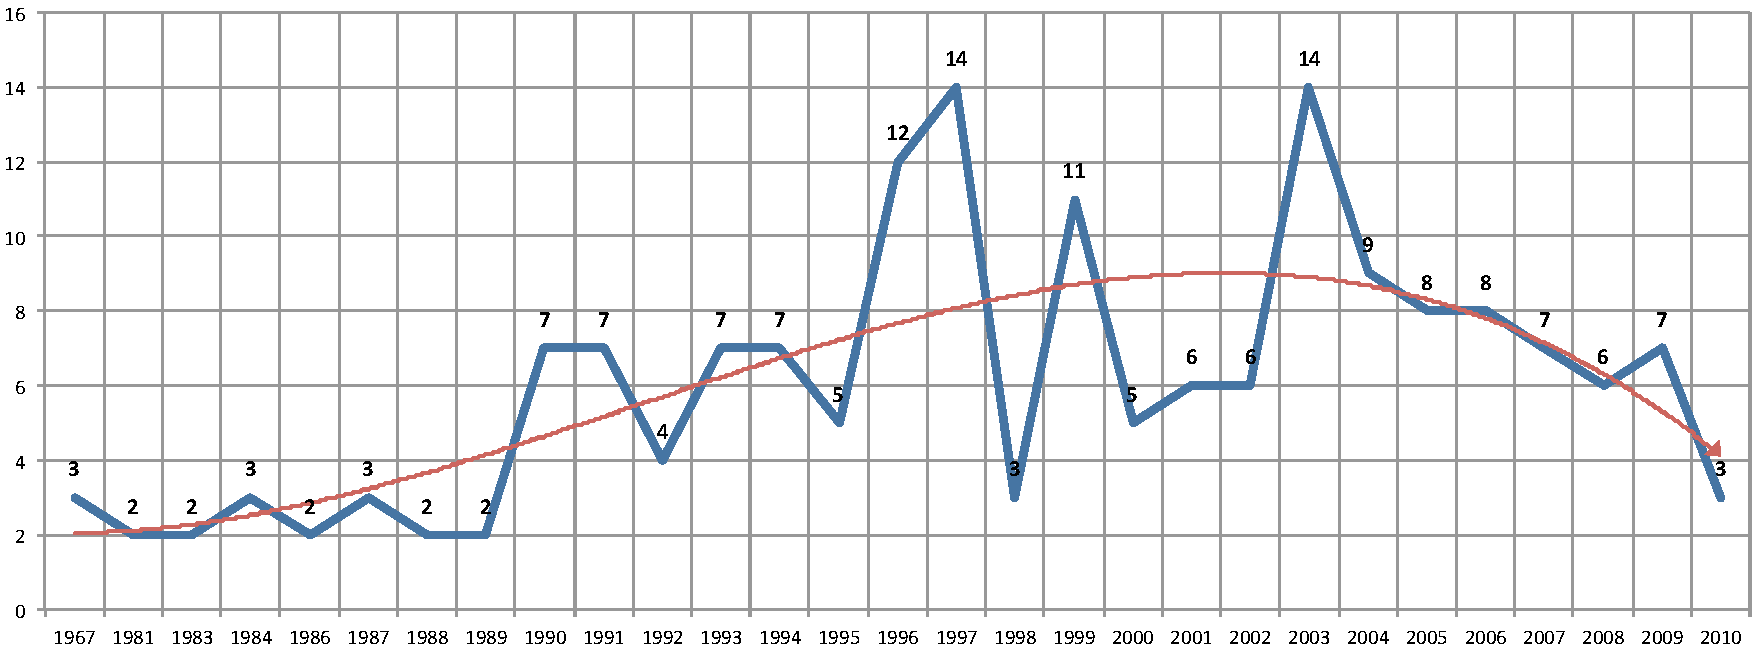
\includegraphics[scale=0.5]{abntex2-modelo-img-grafico.pdf}
	\end{center}
	\legend{Fonte: \citeonline[p. 24]{araujo2012}}
\end{figure}

% ---
\subsection{Figuras em \emph{minipages}}
% ---

\emph{Minipages} são usadas para inserir textos ou outros elementos em quadros
com tamanhos e posições controladas. Veja o exemplo da
\autoref{fig_minipage_imagem1} e da \autoref{fig_minipage_grafico2}.
\begin{figure}[htb]
 \label{teste}
 \centering
  \begin{minipage}{0.45\textwidth}
    \centering
    \caption{Imagem 1 da minipage} \label{fig_minipage_imagem1}
    
\includegraphics[scale=0.8]{abntex2-modelo-img-marca.pdf}
    \legend{Fonte: Produzido pelos autores}
  \end{minipage}
  \hfill
  \begin{minipage}{0.45\textwidth}
    \centering
    \caption{Grafico 2 da minipage} \label{fig_minipage_grafico2}
    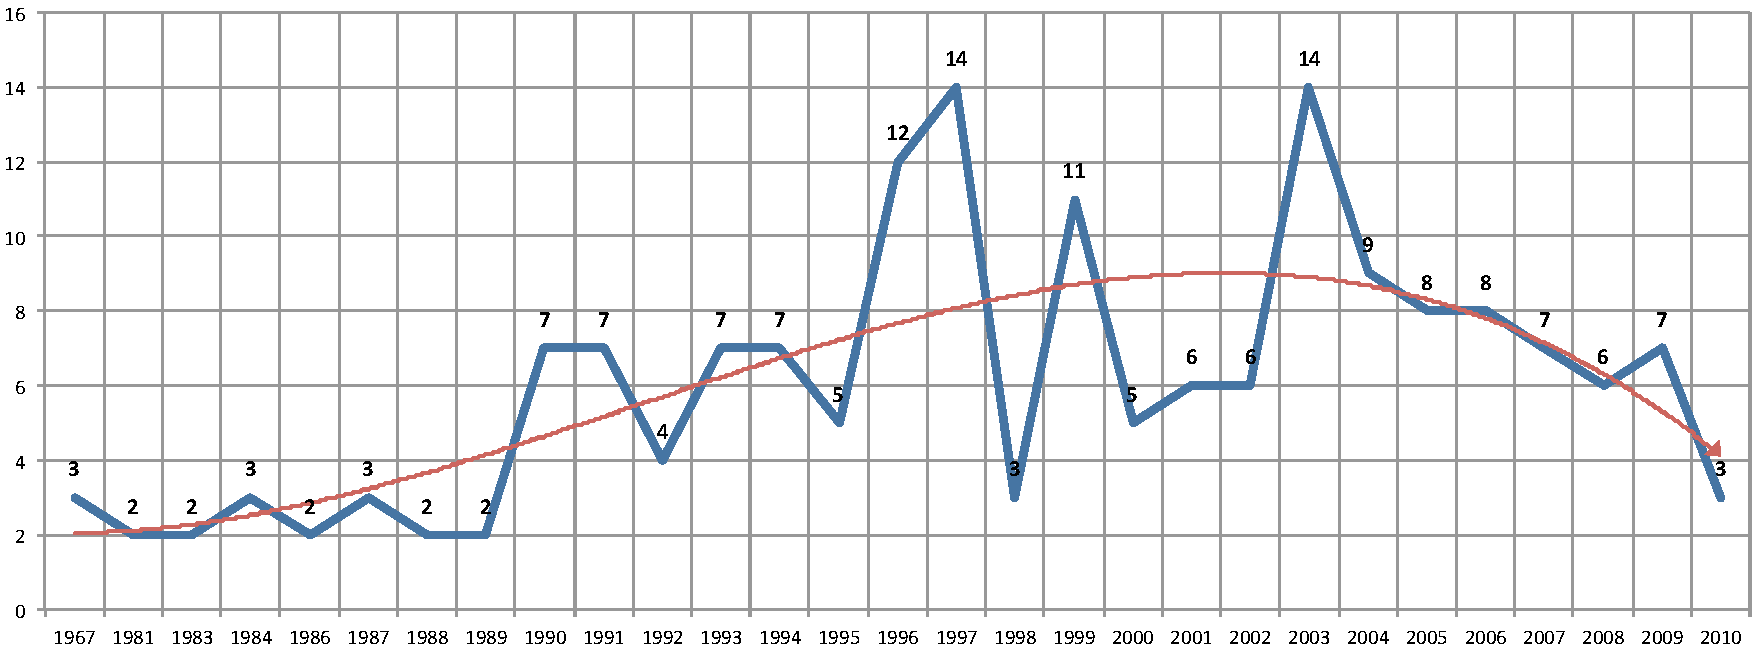
\includegraphics[scale=0.2]{abntex2-modelo-img-grafico.pdf}
    \legend{Fonte: \citeonline[p. 24]{araujo2012}}
  \end{minipage}
\end{figure}

Observe que, segundo a \citeonline[seções 4.2.1.10 e 5.8]{NBR14724:2011}, as
ilustrações devem sempre ter numeração contínua e única em todo o documento:
\begin{citacao}
Qualquer que seja o tipo de ilustração, sua identificação aparece na parte
superior, precedida da palavra designativa (desenho, esquema, fluxograma,
fotografia, gráfico, mapa, organograma, planta, quadro, retrato, figura,
imagem, entre outros), seguida de seu número de ordem de ocorrência no texto,
em algarismos arábicos, travessão e do respectivo título. Após a ilustração, na
parte inferior, indicar a fonte consultada (elemento obrigatório, mesmo que
seja produção do próprio autor), legenda, notas e outras informações
necessárias à sua compreensão (se houver). A ilustração deve ser citada no
texto e inserida o mais próximo possível do trecho a que se
refere. \cite[seção 5.8]{NBR14724:2011}
\end{citacao}

% ---
\section{Subfiguras}
% ---

Como pode ser visto em \citeonline[seção 5.8]{NBR14724:2011}, as subfiguras não 
são elementos regulamentados pelas normas ABNT. A classe \textsf{memoir} dispõe
de comandos para inserção e manejo de subfiguras sem a necessidade de adição de
novos pacotes. Como exemplo, podemos dispor de subfiguras tais como as que seguem
na \autoref{fig_subfigs}, respectivamente as subfiguras \ref{subfig_one} e 
\ref{subfig_two}, juntamente com a \autoref{subfig_three}.
\begin{figure}
  \centering
  \caption{Usando subfiguras}
  \label{fig_subfigs}
  \subtop[\label{subfig_one}Primeira subfigura]{%
    \includegraphics[width=0.3\linewidth]{example-image-a}}
  \subtop[\label{subfig_two}Segunda subfigura]{%
    \includegraphics[width=0.3\linewidth]{example-image-b}}
  \subtop[queisso][\label{subfig_three}Terceira subfigura, com título em mais de uma linha]{%
    \includegraphics[width=0.3\linewidth]{example-image-c}}
  \legend{Fonte: Extraído de \TeX--\LaTeX\ Stack Exchange}
\end{figure}

% ---
\section{Expressões matemáticas}
\label{math-expr}
% ---

\index{expressões matemáticas}Use o ambiente \texttt{equation} para escrever
expressões matemáticas numeradas:
\begin{equation}
  \forall x \in X, \quad \exists \: y \leq \epsilon
\end{equation}

Escreva expressões matemáticas entre \$ e \$, como em $ \lim_{x \to \infty}
\exp(-x) = 0 $, para que fiquem na mesma linha.

Também é possível usar colchetes para indicar o início de uma expressão
matemática que não é numerada.
\[
\left|\sum_{i=1}^n a_ib_i\right|
\le
\left(\sum_{i=1}^n a_i^2\right)^{1/2}
\left(\sum_{i=1}^n b_i^2\right)^{1/2}
\]

Consulte mais informações sobre expressões matemáticas em
\url{https://github.com/abntex/abntex2/wiki/Referencias}.

%---
\section{Teoremas, lemas, proposições e outros ambientes}
% ---

A comunidade matemática utiliza com bastante frequência os ambientes 
\textsf{teorema}, \textsf{lema}, \textsf{proposição} e outros ambientes 
relacionados. Tais definições não necessitam de pacotes adicionais e
podem ser realizadas nas configurações globais.

\begin{definition}[Limite]
  \label{definicao}
  Sejam $f\colon A\rightarrow\mathds{R}$ uma função e $b\in\mathds{R}$ tais 
  que para todo intervalo aberto $I$, contendo $b$, tem-se 
  $I\cap(A-\{b\})\neq\emptyset$. O número real $L$ é o limite de $f(x)$ quando
  $x$ aproxima-se de $b$ quando para todo número $\epsilon>0$, existe $\delta>0$
  ($\delta$ dependendo de $\epsilon$), tal que, se $x\in A$ e $0<|x-b|<\delta$
  então $|f(x)-L|<\epsilon$.
\end{definition}

\begin{proposition}[Unicidade do limnite]
  \label{proposicao}
  Se $\lim_{x\rightarrow b}f(x)=L_1$ e $\lim_{x\rightarrow b}f(x)=L_2$
  ($L_1,L_2\in\mathds{R}$), então $L_1=L_2$.
\end{proposition}

\begin{corollary}
  \label{corolario}
  Se as funções $f(x)$ e $g(x)$ são tais que $f(x) = g(x)$ exceto num ponto $b$,
  então $\lim_{x\rightarrow b}f(x)=\lim_{x\rightarrow b}g(x)$, desde que exista
  um dos limites.
\end{corollary}

\begin{lemma}
  \label{lema}
  Se $a|b$ então $\mathrm{mdc}(a,b)=a$.
\end{lemma}

\begin{theorem}[do Ponto Fixo de Brouwer]
  \label{teorema}
  Se $f\colon[0,1]\rightarrow[0,1]$ é contínua, então $f$ tem ponto fixo.
\end{theorem}
\begin{proof}
  Este ambiente só está definido para o pacote \textsf{amsthm}.
\end{proof}


\begin{conjecture}[de Poincaré]
  \label{conjectura}
  Toda variedade fechada simplesmente conexa de dimensão 3 é equivalente à esfera
  3-dimensional.
\end{conjecture}

% \begin{notation}
%   \label{notacao}
%   oioioi
% \end{notation}

\begin{remark}
  \label{observacao}
  Os gráficos de $f(x) + c$, $f(x + c)$, $cf(x)$ e $f(c x)$ ($c\in\mathds{R}$) 
  podem ser obtidos diretamente do gráfico de $f(x)$.
\end{remark}

% \begin{note}
%   \label{nota}
%   oioioi
% \end{note}

\begin{example}
  \label{exemplo}
  A composta de funções afins é uma função afim.\newline De fato, sejam $f(x)=m_1x+b_1$ e
  $g(x)=m_2x+b_2$. Então, $(g\circ f)(x)=(m_1m_2)x+m_2b_1+b_2$ e 
  $(f\circ g)(x)=(m_1m_2)x+m_1b_2+b_1$.
\end{example}

Para citar no texto, basta usar \textsf{label} dentro de cada ambiente desejado:
\autoref{definicao}, \autoref{proposicao}, \autoref{corolario}, \autoref{lema},
\autoref{teorema}, \autoref{conjectura}, \autoref{observacao}, \autoref{exemplo}.
%, \autoref{}, \autoref{}.

% ---
\section{Enumerações: alíneas e subalíneas}
% ---

\index{alíneas}\index{subalíneas}\index{incisos}Quando for necessário enumerar
os diversos assuntos de uma seção que não possua título, esta deve ser
subdividida em alíneas \cite[4.2]{NBR6024:2012}:
\begin{alineas}
  \item os diversos assuntos que não possuam título próprio, dentro de uma mesma
  seção, devem ser subdivididos em alíneas; 
  
  \item o texto que antecede as alíneas termina em dois pontos;
  \item as alíneas devem ser indicadas alfabeticamente, em letra minúscula,
  seguida de parêntese. Utilizam-se letras dobradas, quando esgotadas as
  letras do alfabeto;

  \item as letras indicativas das alíneas devem apresentar recuo em relação à
  margem esquerda;

  \item o texto da alínea deve começar por letra minúscula e terminar em
  ponto-e-vírgula, exceto a última alínea que termina em ponto final;

  \item o texto da alínea deve terminar em dois pontos, se houver subalínea;

  \item a segunda e as seguintes linhas do texto da alínea começa sob a
  primeira letra do texto da própria alínea;
  
  \item subalíneas \cite[4.3]{NBR6024:2012} devem ser conforme as alíneas a
  seguir:

  \begin{alineas}
     \item as subalíneas devem começar por travessão seguido de espaço;

     \item as subalíneas devem apresentar recuo em relação à alínea;

     \item o texto da subalínea deve começar por letra minúscula e terminar em
     ponto-e-vírgula. A última subalínea deve terminar em ponto final, se não
     houver alínea subsequente;

     \item a segunda e as seguintes linhas do texto da subalínea começam sob a
     primeira letra do texto da própria subalínea.
  \end{alineas}
  
  \item no \abnTeX\ estão disponíveis os ambientes \texttt{incisos} e
  \texttt{subalineas}, que em suma são o mesmo que se criar outro nível de
  \texttt{alineas}, como nos exemplos à seguir:
  
  \begin{incisos}
    \item \textit{Um novo inciso em itálico};
  \end{incisos}
  
  \item Alínea em \textbf{negrito}:
  
  \begin{subalineas}
    \item \textit{Uma subalínea em itálico};
    \item \underline{\textit{Uma subalínea em itálico e sublinhado}}; 
  \end{subalineas}
  
  \item Última alínea com \emph{ênfase}.
  
\end{alineas}

% ---
\section{Espaçamento entre parágrafos e linhas}
% ---

\index{espaçamento!dos parágrafos}O tamanho do parágrafo, espaço entre a margem
e o início da frase do parágrafo, é definido por:
\begin{verbatim}
   \setlength{\parindent}{2.0cm}
\end{verbatim}

\index{espaçamento!do primeiro parágrafo}Por padrão, não há espaçamento no
primeiro parágrafo de cada início de divisão do documento
(\autoref{sec-divisoes}). Porém, você pode definir que o primeiro parágrafo
também seja indentado, como é o caso deste documento. Para isso, apenas inclua o
pacote \textsf{indentfirst} no preâmbulo do documento:
\begin{verbatim}
 \usepackage{indentfirst}    % Indenta o primeiro parágrafo de cada seção.
\end{verbatim}

\index{espaçamento!entre os parágrafos}O espaçamento entre um parágrafo e outro
pode ser controlado por meio do comando:
\begin{verbatim}
  \setlength{\parskip}{0.2cm}  % tente também \onelineskip
\end{verbatim}

\index{espaçamento!entre as linhas}O controle do espaçamento entre linhas é
definido por:
\begin{verbatim}
  \OnehalfSpacing       % espaçamento um e meio (padrão); 
  \DoubleSpacing        % espaçamento duplo
  \SingleSpacing        % espaçamento simples	
\end{verbatim}

Para isso, também estão disponíveis os ambientes:
\begin{verbatim}
  \begin{SingleSpace} ...\end{SingleSpace}
  \begin{Spacing}{hfactori} ... \end{Spacing}
  \begin{OnehalfSpace} ... \end{OnehalfSpace}
  \begin{OnehalfSpace*} ... \end{OnehalfSpace*}
  \begin{DoubleSpace} ... \end{DoubleSpace}
  \begin{DoubleSpace*} ... \end{DoubleSpace*} 
\end{verbatim}

Para mais informações, consulte \citeonline[p. 47-52 e 135]{memoir}.

% ---
\section{Inclusão de outros arquivos}\label{sec-include}
% ---

É uma boa prática dividir o seu documento em diversos arquivos, e não
apenas escrever tudo em um único. Esse recurso foi utilizado neste
documento. Para incluir diferentes arquivos em um arquivo principal,
de modo que cada arquivo incluído fique em uma página diferente, utilize o
comando:
\begin{verbatim}
   \include{documento-a-ser-incluido}      % sem a extensão .tex
\end{verbatim}

Para incluir documentos sem quebra de páginas, utilize:
\begin{verbatim}
   \input{documento-a-ser-incluido}      % sem a extensão .tex
\end{verbatim}

% ---
\section{Compilar o documento \LaTeX}
% ---

Geralmente os editores \LaTeX, como o
TeXlipse\footnote{\url{http://texlipse.sourceforge.net/}}, o
Texmaker\footnote{\url{http://www.xm1math.net/texmaker/}}, entre outros,
compilam os documentos automaticamente, de modo que você não precisa se
preocupar com isso.

No entanto, você pode compilar os documentos \LaTeX usando os seguintes
comandos, que devem ser digitados no \emph{Prompt de Comandos} do Windows ou no
\emph{Terminal} do Mac ou do Linux:
\begin{verbatim}
  pdflatex ARQUIVO_PRINCIPAL.tex
  bibtex ARQUIVO_PRINCIPAL.aux
  makeindex ARQUIVO_PRINCIPAL.idx 
  makeindex ARQUIVO_PRINCIPAL.nlo -s nomencl.ist -o ARQUIVO_PRINCIPAL.nls
  pdflatex ARQUIVO_PRINCIPAL.tex
  pdflatex ARQUIVO_PRINCIPAL.tex
\end{verbatim}

% ---
\section{Remissões internas}
% ---

Ao nomear a \autoref{tab-nivinv} e a \autoref{fig_circulo}, apresentamos
um exemplo de remissão interna que também pode ser feita quando indicamos
o \autoref{cap_exemplos}, que tem o nome \emph{\nameref{cap_exemplos}}.
O número do capítulo indicado é \ref{cap_exemplos}, que se inicia à
\autopageref{cap_exemplos}\footnote{O número da página de uma remissão
pode ser obtida também assim:
\pageref{cap_exemplos}.}.
Veja a \autoref{sec-divisoes} para outros exemplos de remissões internas
entre seções, subseções e subsubseções.

O código usado para produzir o texto desta seção é:
\begin{verbatim}
Ao nomear a \autoref{tab-nivinv} e a \autoref{fig_circulo}, apresentamos
um exemplo de remissão interna que também pode ser feita quando indicamos
o \autoref{cap_exemplos}, que tem o nome \emph{\nameref{cap_exemplos}}.
O número do capítulo indicado é \ref{cap_exemplos}, que se inicia à
\autopageref{cap_exemplos}\footnote{O número da página de uma remissão
pode ser obtida também assim:
\pageref{cap_exemplos}.}.
Veja a \autoref{sec-divisoes} para outros exemplos de remissões internas
entre seções, subseções e subsubseções.
\end{verbatim}

% ---
\section{Divisões do documento: seção}\label{sec-divisoes}
% ---

Esta seção testa o uso de divisões de documentos. Esta é a
\autoref{sec-divisoes}. Veja a \autoref{sec-divisoes-subsection}.

\subsection{Divisões do documento: subseção}\label{sec-divisoes-subsection}

Isto é uma subseção. Veja a \autoref{sec-divisoes-subsubsection}, que é uma
\texttt{subsubsection} do \LaTeX, mas é impressa chamada de ``subseção'' porque
no Português não temos a palavra ``subsubseção''.

\subsubsection{Divisões do documento: subsubseção}
\label{sec-divisoes-subsubsection}

Isto é uma subsubseção.

\subsubsection{Divisões do documento: subsubseção}

Isto é outra subsubseção.

\subsection{Divisões do documento: subseção}\label{sec-exemplo-subsec}

Isto é uma subseção.

\subsubsection{Divisões do documento: subsubseção}

Isto é mais uma subsubseção da \autoref{sec-exemplo-subsec}.


\subsubsubsection{Esta é uma subseção de quinto
nível}\label{sec-exemplo-subsubsubsection}

Esta é uma seção de quinto nível. Ela é produzida com o seguinte comando:
\begin{verbatim}
\subsubsubsection{Esta é uma subseção de quinto
nível}\label{sec-exemplo-subsubsubsection}
\end{verbatim}

\subsubsubsection{Esta é outra subseção de quinto nível}\label{sec-exemplo-subsubsubsection-outro}

Esta é outra seção de quinto nível.


\paragraph{Este é um parágrafo numerado}\label{sec-exemplo-paragrafo}

Este é um exemplo de parágrafo nomeado. Ele é produzida com o comando de
parágrafo:
\begin{verbatim}
\paragraph{Este é um parágrafo nomeado}\label{sec-exemplo-paragrafo}
\end{verbatim}

A numeração entre parágrafos numeradaos e subsubsubseções são contínuas.

\paragraph{Esta é outro parágrafo numerado}\label{sec-exemplo-paragrafo-outro}

Esta é outro parágrafo nomeado.

% ---
\section{Este é um exemplo de nome de seção longo. Ele deve estar
alinhado à esquerda e a segunda e demais linhas devem iniciar logo abaixo da
primeira palavra da primeira linha}
% ---

Isso atende à norma \citeonline[seções de 5.2.2 a 5.2.4]{NBR14724:2011} 
 e \citeonline[seções de 3.1 a 3.8]{NBR6024:2012}.

% ---
\section{Diferentes idiomas e hifenizações}
\label{sec-hifenizacao}
% ---

Para usar hifenizações de diferentes idiomas, inclua nas opções do documento o
nome dos idiomas que o seu texto contém. Por exemplo (para melhor
visualização, as opções foram quebras em diferentes linhas):
\begin{verbatim}
\documentclass[
	12pt,
	openright,
	twoside,
	a4paper,
	english,
	spanish,
	brazil
	]{abntex2}
\end{verbatim}

O idioma português-brasileiro (\texttt{brazil}) é incluído automaticamente pela
classe \textsf{abntex2}. Porém, mesmo assim a opção \texttt{brazil} deve ser
informada como a última opção da classe para que todos os pacotes reconheçam o
idioma. Vale ressaltar que a última opção de idioma é a utilizada por padrão no
documento. Desse modo, caso deseje escrever um texto em inglês que tenha
citações em português e em espanhol, você deveria usar o preâmbulo como abaixo:
\begin{verbatim}
\documentclass[
	12pt,
	openright,
	twoside,
	a4paper,
	spanish,
	brazil,
	english
	]{abntex2}
\end{verbatim}

A lista completa de idiomas suportados, bem como outras opções de hifenização,
estão disponíveis em \citeonline[p.~5-6]{babel}.

Exemplo de hifenização em inglês\footnote{Extraído de:
\url{http://en.wikibooks.org/wiki/LaTeX/Internationalization}}:

\begin{otherlanguage*}{english}
\textit{Text in English language. This environment switches all language-related
definitions, like the language specific names for figures, tables etc. to the other
language. The starred version of this environment typesets the main text
according to the rules of the other language, but keeps the language specific
string for ancillary things like figures, in the main language of the document.
The environment hyphenrules switches only the hyphenation patterns used; it can
also be used to disallow hyphenation by using the language name
`nohyphenation'.}
\end{otherlanguage*}

% Pequeno texto em espanhol\footnote{Extraído de:
% \url{http://internacional.elpais.com/internacional/2013/02/17/actualidad/1361102009_913423.html}}:
% 
% \foreignlanguage{spanish}{\textit{Decenas de miles de personas ovacionan al pontífice en su
% penúltimo ángelus dominical, el primero desde que anunciase su renuncia. El Papa se
% centra en la crítica al materialismo}}.

O idioma geral do texto por ser alterado como no exemplo seguinte:
\begin{verbatim}
  \selectlanguage{english}
\end{verbatim}

Isso altera automaticamente a hifenização e todos os nomes constantes de
referências do documento para o idioma inglês. Consulte o manual da classe
\cite{abntex2classe} para obter orientações adicionais sobre internacionalização de
documentos produzidos com \abnTeX.

A \autoref{sec-citacao} descreve o ambiente \texttt{citacao} que pode receber
como parâmetro um idioma a ser usado na citação.

% ---
\section{Consulte o manual da classe \textsf{abntex2}}
% ---

Consulte o manual da classe \textsf{abntex2} \cite{abntex2classe} para uma
referência completa das macros e ambientes disponíveis. 

Além disso, o manual possui informações adicionais sobre as normas ABNT
observadas pelo \abnTeX\ e considerações sobre eventuais requisitos específicos
não atendidos, como o caso da \citeonline[seção 5.2.2]{NBR14724:2011}, que
especifica o espaçamento entre os capítulos e o início do texto, regra
propositalmente não atendida pelo presente modelo.

% ---
\section{Referências bibliográficas}
% ---

A formatação das referências bibliográficas conforme as regras da ABNT são um
dos principais objetivos do \abnTeX. Consulte os manuais
\citeonline{abntex2cite} e \citeonline{abntex2cite-alf} para obter informações
sobre como utilizar as referências bibliográficas.

ATENÇÃO: a utilização do comando \textsf{citeonline} em vez de \textsf{cite} só
é permitida quando utiliza-se o pacote \textsf{abntex2cite}!

%-
\subsection{Acentuação de referências bibliográficas}
%-

Normalmente não há problemas em usar caracteres acentuados em arquivos
bibliográficos (\texttt{*.bib}). Porém, como as regras da ABNT fazem uso quase
abusivo da conversão para letras maiúsculas, é preciso observar o modo como se
escreve os nomes dos autores. Na ~\autoref{tabela-acentos} você encontra alguns
exemplos das conversões mais importantes. Preste atenção especial para `ç' e `í'
que devem estar envoltos em chaves. A regra geral é sempre usar a acentuação
neste modo quando houver conversão para letras maiúsculas.
\begin{table}[htbp]
\caption{Tabela de conversão de acentuação.}
\label{tabela-acentos}
\begin{center}
\begin{tabular}{ll}\hline\hline
acento & \textsf{bibtex}\\
à á ã & \verb+\`a+ \verb+\'a+ \verb+\~a+\\
í & \verb+{\'\i}+\\
ç & \verb+{\c c}+\\
\hline\hline
\end{tabular}
\end{center}
\end{table}

% ---
\section{Referências cruzadas (cross referencing)}
% ---

A classe \abnTeX\ permite o uso do comando \textsf{autoref} para referenciar 
diversos itens do texto produzido, como capítulos e seções, figuras, tabelas, 
equações, algoritmos e códigos. A partir de um \textsf{label} fornecido, basta 
utilizar o comando para referenciar algo do texto.

Como exemplo, podemos citar a \autoref{tabela-acentos}, a 
\autoref{fig_grafico}, a \autoref{math-expr} e o \autoref{chpt2}.
Sem o \textsf{autoref} a saída se torna a Tabela 
\ref{tabela-acentos}, a Figura \ref{fig_grafico}, a seção 
\ref{math-expr} e o Capítulo \ref{chpt2}.

O código que gerou o parágrafo anterior foi:
\begin{verbatim}
Como exemplo, podemos citar a \autoref{tabela-acentos}, a 
\autoref{fig_grafico}, a \autoref{math-expr} e o \autoref{chpt2}.
Sem o \textsf{autoref} a saída se torna a Tabela 
\ref{tabela-acentos}, a Figura \ref{fig_grafico}, a seção 
\ref{math-expr} e o Capítulo \ref{chpt2}.
\end{verbatim}

Perceba a necessidade de inserir o label a que se refere a referência
(Tabela, Figura, Capítulo) quando não usamos o comando \textsf{autoref}.


% ----------------------------------------------------------
% ----------------------------------------------------------

\part{Referenciais teóricos}

% ----------------------------------------------------------
% Este capítulo ilustra o uso de glossarios com a classe abnTeX2
% ----------------------------------------------------------
% ----------------------------------------------------------
% ----------------------------------------------------------

\chapter{Orientações a respeito de glossários}
\label{chpt2}
 
% ---
\section{Usar o glossário no texto}
% ---
 
Você pode definir as entradas do glossário no início do texto. Recomenda-se o
uso de um arquivo separado a ser inserido ainda no preâmbulo. Veja orientações
sobre inclusão de arquivos na \autoref{sec-include}.

No decorrer do texto, use os termos do glossário como na frase:

\begin{citacao}
Esta frase usa a palavra \gls{componente} e o plural de \glspl{filho},
ambas definidas no glossário como filhas da entrada \gls{pai}.
\Gls{equilibrio} exemplifica o uso de um termo no início da frase. O
software \gls{abntex2} é escrito em \gls{latex}, que é definido no
glossário como \emph{`\glsdesc*{latex}'}.
\end{citacao}


A frase acima foi produzida com:
\begin{verbatim}
Esta frase usa a palavra \gls{componente} e o plural de \glspl{filho},
ambas definidas no glossário como filhas da entrada \gls{pai}.
\Gls{equilibrio} exemplifica o uso de um termo no início da frase. O
software \gls{abntex2} é escrito em \gls{latex}, que é definido no
glossário como \emph{`\glsdesc*{latex}'}.
\end{verbatim}

Opcionalmente, incorpore todas as palavras do glossário de uma única vez ao
documento com o comando 
\begin{verbatim}
   \glsaddall
\end{verbatim}
 
A impressão efetiva do glossário é dada com:
\begin{verbatim}
   \printglossaries
\end{verbatim}

A impressão do glossário incorpora o número das páginas em que as entradas foram
citadas. Isso pode ser removido adicionando-se a opção \texttt{nonumberlist} em:
\begin{verbatim}
\usepackage[nonumberlist,style=index]{glossaries}%
\end{verbatim}

% ---
\section{Compilar um documento com glossário}
\label{sec-compilar-glossario}
% ---
 
Para compilar um documento \LaTeX\ com glossário use:
\begin{verbatim}
  pdflatex ARQUIVO_PRINCIPAL.tex
  bibtex ARQUIVO_PRINCIPAL.aux
  makeindex ARQUIVO_PRINCIPAL.idx 
  makeindex ARQUIVO_PRINCIPAL.nlo -s nomencl.ist -o ARQUIVO_PRINCIPAL.nls
  makeglossaries ARQUIVO_PRINCIPAL.aux
  pdflatex ARQUIVO_PRINCIPAL.tex
  pdflatex ARQUIVO_PRINCIPAL.tex
\end{verbatim}
 
O comando \texttt{makeglossaries} é um aplicativo Perl instalado
automaticamente pelas distribuições MacTeX, TeX Live e MiKTeX. Geralmente
usuários de Linux e de Mac OS X já possuem o interpretador Perl\footnote{O Perl
é uma linguagem de programação de scripts muito utilizada pela comunidade de
software livre. Veja o site do projeto em \url{http://www.perl.org/}.} instalado
e configurado e nenhuma configuração adicional é necessária.

Usuários de Windows, por outro lado, precisam instalar a ferramenta Perl para
que seja possível usar \texttt{makeglossaries}. Por sorte isso é simples. Para
obter a instalação do Perl para seu sistema operacional visite \url{http://www.perl.org/get.html}.

Alternativamente ao aplicativo Perl \texttt{makeglossaries}, é possível usar o
aplicativo \texttt{makeglossariesgui}\footnote{O título do aplicativo no CTAN
é \textit{Java GUI alternative to makeglossarires script}.}, que possui uma
interface gráfica baseada em Java. Para isso, consulte
\url{http://www.ctan.org/pkg/makeglossariesgui}. Funciona em Windows,
Linux e Mac OS X.

% ---
\section{Configuração de glossários}
% ---

O pacote \textsf{glossaries}, usado na produção dos glossários deste exemplo,
possui diversas configurações. É possível alterar o estilo da impressão do
glossário, criar campos adicionais, usar diversos glossários em
arquivos separados. Para isso e outras informações, consulte a documentação do
pacote \textsf{glossaries}: \url{http://www.ctan.org/pkg/glossaries}.

Consulte também o livro da WikiBooks sobre a produção de glossários:
\url{http://en.wikibooks.org/wiki/LaTeX/Glossary}.
 

\subsection{Estilos do glossário}

O pacote \textsf{glossaries} traz dezenas de estilos pré-definidos de
glossários. Eles estão disponíveis no capítulo 15 do manual do pacote
\cite{talbot2012}. O capítulo 16 contém instruções sobre como criar um estilo
personalizado.

Os estilos podem ser alterados com:
\begin{verbatim}
   \setglossarystyle{altlisthypergroup}
\end{verbatim}

O estilo \texttt{index} é ideal para construção de glossários com diversos
níveis hierárquicos do tipo pai-filho. Já o modelo \texttt{altlisthypergroup} é
mais adequado para glossários sem hierarquias. Teste também o modelo
\texttt{tree}.

Se desejar um único estilo de glossário padrão no documento, alternativamente
inclua a opção \texttt{style} nas opções da classe, do
seguinte modo:

\begin{verbatim}
   \usepackage[style=index]{glossaries}
\end{verbatim}

% ---
\section{Problemas com a ordem das palavras?}
% ---

Este exemplo do \abnTeX\ utiliza a ferramenta \texttt{makeindex} -- padrão das
distribuições \LaTeX\ mais comuns -- para ordenar as entradas do glossário.
Porém, essa ferramenta não possui opções de \textit{collation} e não funciona
bem para palavras escritas em idiomas que não sejam inglês.
Por isso, pode acontecer que letras acentuadas e outros caracteres
internacionais sejam ordenados de forma incorreta, como no exemplo (palavras não
necessariamente presentes na língua portuguesa):

\begin{alineas}
 \item Amor: ...
 \item Aviar: ...
 \item Avião: ...
 \item Aço: ...
\end{alineas}

Por sorte, é possível substituir o uso do \texttt{makeindex}
pelo \texttt{xindy}\footnote{\url{http://www.xindy.org/}}. Para isso, faça o
seguinte:

\begin{alineas}
  \item Certifique-se de que o Xindy esteja instalado. Em um terminal, digite:
  \texttt{xindy --version}\footnote{Caso o Xindy não esteja presente no sistema,
    é necessário instalá-lo. Usuários Linux Debian/Ubuntu podem usar: 
    \texttt{sudo apt-get install xindy}. Usuários Windows e Mac podem acessar
    a página do Xindy, baixá-lo e instalá-lo.};
  \item No código LaTeX, ainda no preâmbulo, inclua a seguinte opção ao pacote glossaries:
  \indent
  \begin{verbatim}
  \usepackage[xindy={language=portuguese},
                     nonumberlist=true]{glossaries}
  \end{verbatim}
  \item Compile o glossário normalmente, conforme a
  \autoref{sec-compilar-glossario}.
\end{alineas}


% ----------------------------------------------------------
% ----------------------------------------------------------

\part{Resultados}

% ----------------------------------------------------------
% ----------------------------------------------------------
% ----------------------------------------------------------

% ---
\chapter{Algoritmos e códigos-fonte}
% ---

\section{O pacote algorithm2e}

O \textsf{algorithm2e} é um ambiente para escrever algoritmos. Um algoritmo se 
torna um objeto flutuante (como uma figura, tabela, etc.).

\begin{algorithm}
\caption{Primeiro exemplo de algoritmo com uma legenda contendo um texto muito longo que pode ocupar mais de uma linha.\label{IR}}
\KwData{$G=(X,U)$ such that $G^{tc}$ is an order.}
\KwResult{$G'=(X,V)$ with $V\subseteq U$ such that $G'^{tc}$ is an interval order.}
\Begin{
    $V \longleftarrow U$\;
    $S \longleftarrow \emptyset$\;
    \For{$x\in X$}{
	$NbSuccInS(x) \longleftarrow 0$\;
	$NbPredInMin(x) \longleftarrow 0$\;
	$NbPredNotInMin(x) \longleftarrow |ImPred(x)|$\;
    }
    \For{$x \in X$}{
	\If{$NbPredInMin(x) = 0$ \textnormal{\textbf{and}} $NbPredNotInMin(x) = 0$}{$AppendToMin(x)$}
    }
    \nl\While{$S \neq \emptyset$}{\label{InRes1}
	\nlset{REM} remove $x$ from the list of $T$ of maximal index\;\label{InResR}
	\lnl{InRes2}\While{$|S \cap  ImSucc(x)| \neq |S|$}{
	    \For{$ y \in  S-ImSucc(x)$}{
		\{ remove from $V$ all the arcs $zy$ : \}\;
		\For{$z \in  ImPred(y) \cap  Min$}{
		    remove the arc $zy$ from $V$\;
		    $NbSuccInS(z) \longleftarrow NbSuccInS(z) - 1$\;
		    move $z$ in $T$ to the list preceding its present list\;
		    \{i.e. If $z \in T[k]$, move $z$ from $T[k]$ to
		    $T[k-1]$\}\;
		}
		$NbPredInMin(y) \longleftarrow 0$\;
		$NbPredNotInMin(y) \longleftarrow 0$\;
		$S \longleftarrow S - \{y\}$\;
		$AppendToMin(y)$\;
	    }
	}
	$RemoveFromMin(x)$\;
    }
}
\end{algorithm}

Como pode ser visto na documentação do pacote \textsf{algorithm2e} (informações
em  \url{https://www.ctan.org/pkg/algorithm2e}), o pacote não oferece comandos 
para quebra de página, caso seu algoritmo ocupe mais de uma página. Em muitos
casos, este inconveniente pode ser facilmente contornado alterando o tamanho a
fonte utilizada no ambiente. O ponto forte deste pacote é que ele é um pacote 
que  possui atualizações periódicas, sendo a última versão a 5.1 datada de 10 
de novembro de 2015 (Manter todo o sistema \LaTeX\ atualizado é vital para o 
bom funcionamento de todos os pacotes e comandos utilizados: mantenha seu 
sistema sempre atualizado!).

\setcounter{algocf}{98}

\begin{algorithm}
\SetAlgoLined
\KwData{this text}
\KwResult{how to write algorithm with \LaTeX2e }
initialization\;
\While{not at end of this document}{
read current\;
\eIf{understand}{
go to next section\;
current section becomes this one\;
}{
go back to the beginning of current section\;
}
}
\caption{How to write algorithms.}
\end{algorithm}

\section{O pacote listings}

O pacote permite que o usuário escreva programas (código de programação) dentro
do \LaTeX; O código-fonte é lido diretamente pelo TeX-nenhum processador front-end
é necessário. Palavras-chave, comentários e seqüências de caracteres podem ser 
composta usando estilos diferentes (padrão é negrito para palavras-chave, itálico
para comentários e nenhum estilo especial para seqüências de caracteres). Suporte
para hyperref é fornecido (informações em \url{https://www.ctan.org/pkg/listings}).

\begin{lstlisting}[caption={Exemplo de código em C++ usando o pacote \texttt{listings} e que tem título longo ocupando mais de uma linha},label=ex-listing]
#include 
using namespace std;
int main()
{
  /* comentario */
  int n, i, a = 0, b = 1, F;
  cout << "Digite o numero de termos da sequencia de Fibonacci: ";
   cin >> n;
  cout << a << " " << b << " ";
   for (i = 0; i < n - 2; i++)   {
     F = a + b;
     cout << F << " ";
     a = b;
     b = F;
   } cout << endl; return 0;
 }
\end{lstlisting}

Diferentemente do pacote \textsf{algorithm2e}, o pacote \textsf{listings} não
possui problemas com quebra de páginas para códigos computacionais que ocupem
mais de uma página.

\setcounter{lstlisting}{98}

\begin{lstlisting}[caption=Exemplo de código em C++ usando o pacote \texttt{listings},label=ex-listing-two]
#include 
using namespace std;
int main()
{
  /* comentario */
  int n, i, a = 0, b = 1, F;
  cout << "Digite o numero de termos da sequencia de Fibonacci: ";
   cin >> n;
  cout << a << " " << b << " ";
   for (i = 0; i < n - 2; i++)   {
     F = a + b;
     cout << F << " ";
     a = b;
     b = F;
   } cout << endl; return 0;
 }
\end{lstlisting}
% ---
% --------------------
% FIM DOS EXEMPLOS
% --------------------
% ----------------------------------------------------------
% CONSIDERAÇÕES FINAIS
% Finaliza a parte no bookmark do PDF para que se inicie o
% bookmark na raiz e adiciona espaço de parte no Sumário
\phantompart
\include{considfinais}
% ----------------------------------------------------------
% ---------------------------------------------------------------------------------
% %%%%%%%%%%%%%%%%%%%%%%%%%% FIM DOS ELEMENTOS TEXTUAIS %%%%%%%%%%%%%%%%%%%%%%%%%%
% ---------------------------------------------------------------------------------
% ---------------------------------------------------------------------------------
% %%%%%%%%%%%%%%%%%%%%%%% INÍCIO DOS ELEMENTOS PÓS-TEXTUAIS %%%%%%%%%%%%%%%%%%%%%%%
% ---------------------------------------------------------------------------------
% ----------------------------------------------------------
\postextual
% ----------------------------------------------------------
% ----------------------------------------------------------
% REFERÊNCIAS
\bibliography{abntex2-modelo-references}
% ----------------------------------------------------------
% ----------------------------------------------------------
% ---------------------------------------------------------------------------------
% %%%%%%%%%%%%%%%%%%%%%%%%%% FIM DOS ELEMENTOS TEXTUAIS %%%%%%%%%%%%%%%%%%%%%%%%%%
% ----------------------------------------------------------------------------------
% -----------------------------------------------------------------------------------------------
% %%%%%%%%%%%%%%%%%%%%%%%%%%%%%%%%%%%%%% FIM DO DOCUMENTO %%%%%%%%%%%%%%%%%%%%%%%%%%%%%%%%%%%%%%
% -----------------------------------------------------------------------------------------------
\end{document}

% Remove caixa alta e deixa tudo do mesmo tamanho no sumário
